\chapter{函数}

\section{基础概念}
\noindent \textbf{关键词}:定义域,值域,单调性,奇偶性(轴对称与中心对称),周期性($ f(x)=f(x+T) $),零点,极值(点),渐近线。 

\begin{itemize}[leftmargin=\inteval{\myitemleftmargin}pt,itemsep=
   \inteval{\myitemitempsep}pt,topsep=\inteval{\myitemtopsep}pt]
\item 零点:使$ f(x)=0 $的$ x $. 
\item 极值点:设函数$ f(x) $在区间$ I $上有定义,$ x_0\in I $,若$ \exists\ \sigma>0,\ \forall\ x\in(x_0-\sigma,x_0+\sigma) $\footnote{$ \exists $表示存在,可以理解为Exist的首字母E左右颠倒;$ \forall $表示任意,可以理解为Any的首字母A上下颠倒。},有$ f(x)\leq f(x_0) $(或$ f(x)\geq f(x_0) $),则称$ f(x_0) $是函数$ f(x) $的一个极大值(或极小值),$ x_0 $是函数的一个极大值点(或极小值点),但有时候也把$ (x_0,f(x_0)) $称为极大值点(或极小值点)。极大值与极小值统称为极值;极大值点与极小值点统称为极值点。高中阶段基本只考察连续、可导的函数,可以认为极值只会在$ f'(x)=0 $的位置取得。
% \item 极点(pole)$ ^* $:使$ f(x)\to +\infty $或$-\infty $的$ x $,比如$ x=0 $是$ \dfrac{1}{x^2} $的极点\footnote{可查阅https://complex-analysis.com/content/classification\_of\_singularities.html,或者\ 胡嗣柱,倪光炯. 数学物理方法[M]. 高等教育出版社,2002. }。

\item 定义域主要考点:\\
(1)分母不为0;\\
(2)对数函数$ \log_a() $括号内的表达式大于0,$a>0$且$ a\neq 1 $;\\
(3)指数函数$a^x$,$a>0$且$ a\neq 1 $;\\
(4)偶数次根式(主要是二次根式)下的表达式大于等于0;\\
(5)正切函数$ \tan() $括号内的表达式不等于$ k\pi+\dfrac{\pi}{2}\ 
(k\in \mathbf{Z}) $. 

\end{itemize}

\section{值域} 
\begin{itemize}[leftmargin=\inteval{\myitemleftmargin}pt,itemsep=
   \inteval{\myitemitempsep}pt,topsep=\inteval{\myitemtopsep}pt]
\item 一般的三次曲线是指形如下式的曲线:
\begin{gather*}
    a_{30}x^3+a_{21}x^2y+a_{12}xy^2+a_{03}y^3+b_{20}x^2+b_{11}xy+b_{02}y^2+
    c_{10}x+c_{01}y+d=0
\end{gather*}
其中,$ a_{30},a_{21},a_{12},a_{03} $不全为0. 三次曲线种类繁多\footnote{陈谷新. 
    平面三次代数曲线\ 连载No.1$ \sim $No.8[J]. (工程)图学学报, 1988年起。},
在此不做详细介绍。

\item 求$ y=\dfrac{Ax+B}{Cx+D} $的值域:
\begin{align}\label{分子分母化为首1多项式}
    \dfrac{Ax+B}{Cx+D} =
    \dfrac{A}{C}\cdot\dfrac{x+\dfrac{D}{C}-\dfrac{D}{C}+\dfrac{B}{A}}
    {x+\dfrac{D}{C}}=\dfrac{A}{C}\cdot
    \left(1+\dfrac{-\dfrac{D}{C}+\dfrac{B}{A}}{x+\dfrac{D}{C}}\right)
\end{align}
求$ y=\dfrac{A\sin x+B}{C\sin x+D}$和$ y=\dfrac{Aa^x+B}{Ca^x+D}$的值域的方法同上。

\item 求$ y=\dfrac{x^2+Ax+B}{x+C} $或$ y=\dfrac{x+C}{x^2+Ax+B} $的值域:\\
若分子或分母的最高次项系数不为1,可以像(\ref{分子分母化为首1多项式})式一样,
通过提取公因数化为1. \\
\textbf{方法一}\ 做代换$ t=x+C $,那么$ x=t-C $,
\begin{align*}
    \dfrac{x^2+Ax+B}{x+C}=&\ \dfrac{(t-C)^2+A(t-C)+B}{t}\\
    =&\ \dfrac{t^2+(A-2C)t+C^2-AC+B}{t}=t+(A-2C)+\dfrac{C^2-AC+B}{t}
\end{align*}
问题就转化成了求关于$ t $的双曲线的值域,可能是双钩函数,也可能是无极值的函数。\\
\textbf{方法二}\ 判别式,$ y(x+C)=x^2+Ax+B,\ x^2+(A-y)x+(B-yC)=0 $,
\begin{align*}
    \Delta=(A-y)^2-4(B-yC)=y^2+(4C-2A)y+A^2-4B\geq 0 
\end{align*}
\textbf{注}:$ y=\dfrac{x+C}{x^2+Ax+B} $属于三次曲线,因为它可以变形为$ y(x^2+Ax+B)-x-C=0 $. 

\item 求$ y=\dfrac{x^2+Ax+B}{x^2+Cx+D} $(属于三次曲线)的值域:
\begin{align*}
    \dfrac{x^2+Ax+B}{x^2+Cx+D} =&\  \dfrac{x^2+Cx+D+(A-C)x+(B-D)}{x^2+Cx+D} \\
    =&\ 1+\dfrac{(A-C)x+(B-D)}{x^2+Cx+D}  \\
    =&\ \begin{cases}
         1+\dfrac{B-D}{x^2+Cx+D} & (A = C) \\
         1+(A-C)\dfrac{x+\dfrac{B-D}{A-C}}{x^2+Cx+D} & (A\neq C)
    \end{cases}
\end{align*}
再做代换$ t=x+\dfrac{B-D}{A-C} $即可。当然也可以直接使用判别式法。

\item 求$ y=\dfrac{x+A}{\sqrt{x^2+Cx+D}} $的值域:\\
\textbf{方法一}\ 考虑$ y^2=\dfrac{x^2+2Ax+A^2}{x^2+Cx+D}
=1+\dfrac{(2A-C)x+(A^2-D)}{x^2+Cx+D} $. \\
\textbf{方法二}\ 做代换$ t=x+A $,那么$ x=t-A $,
\begin{align*}
    y=\dfrac{t}{\sqrt{(t-A)^2+C(t-A)+D}}=&\ \dfrac{t}{\sqrt{t^2+(C-2A)t+A^2-AC+D}} \\
    =&\  \pm \dfrac{1}{\sqrt{1+(C-2A)\dfrac{1}{t}+(A^2-AC+D)\dfrac{1}{t^2}}}
\end{align*}
其中,$ 1+(C-2A)\dfrac{1}{t}+(A^2-AC+D)\dfrac{1}{t^2} $是一个关于$ \dfrac{1}{t} $
的二次函数,容易求出值域。

\item 求$ y= \dfrac{Ax-\sqrt{Bx^2+C}}{Ax+\sqrt{Bx^2+C}} $的值域:\\
\textbf{方法一}
\begin{align*}
    \dfrac{Ax-\sqrt{Bx^2+C}}{Ax+\sqrt{Bx^2+C}} =&\  
    \dfrac{Ax+\sqrt{Bx^2+C}-2\sqrt{Bx^2+C}}{Ax+\sqrt{Bx^2+C}} \\
    =&\  1-\dfrac{2\sqrt{Bx^2+C}}{Ax+\sqrt{Bx^2+C}} \\
    =&\  1-\dfrac{2}{\dfrac{Ax}{\sqrt{Bx^2+C}}+1} \\
    =&\  1-\dfrac{2}{\dfrac{\pm A}{\sqrt{B+\dfrac{C}{x^2}}}+1} 
\end{align*}
$ A $前面的正负号取决于$ x $的正负。\\
\textbf{方法二}
\begin{align*}
    y+\dfrac{1}{y}=&\ \dfrac{Ax-\sqrt{Bx^2+C}}{Ax+\sqrt{Bx^2+C}}+
    \dfrac{Ax+\sqrt{Bx^2+C}}{Ax-\sqrt{Bx^2+C}}   \\
    =&\ \dfrac{2(A^2+B^2)x^2+2C}{(A^2-B^2)x^2+C} \\
    =&\ \dfrac{2(A^2+B^2)}{A^2-B^2}\cdot
    \dfrac{x^2+\dfrac{C}{A^2+B^2}}{x^2+\dfrac{C}{A^2-B^2}} \\
    =&\ \dfrac{2(A^2+B^2)}{A^2-B^2}\cdot \left(1+
    \dfrac{\dfrac{C}{A^2+B^2}-\dfrac{C}{A^2-B^2}}{x^2+\dfrac{C}{A^2-B^2}} \right)
\end{align*}
先求出$ y+\dfrac{1}{y} $的范围,再求$ y $的范围。\\
\textbf{方法三}\ 判别式
\begin{gather*}
    yAx+y\sqrt{Bx^2+C}=Ax-\sqrt{Bx^2+C} \\
    (y+1)\sqrt{Bx^2+C}=Ax(1-y)  \\
    [B(y+1)^2-A^2(1-y)^2]x^2+C(y+1)^2=0 \\
    \Delta =-4[B(y+1)^2-A^2(1-y)^2]C(y+1)^2\geq 0
\end{gather*}
先求解方程$ (B-A^2)y^2+2(B+A^2)y+(B-A^2)=0 $,然后根据$ C $的正负决定区间。

% ABS_Plot.m
\item 函数$ y=|x-b_1|+|x-b_2| $的最小值在区间$ [b_1,b_2] $内取得(假设$ b_1<
b_2 $),在此区间内,函数值为常数$ b_2-b_1 $. 函数$ y=|x-b_1|+|x-b_2|+|x-b_3| $
的最小值在$ x=b_2 $处取得(假设$ b_1<b_2<b_3 $),最小值为$ b_3-b_1 $. 
更一般地,对于$ y=|x-b_1|+|x-b_2|+\cdots+|x-b_n| $,假设$ b_1<b_2<\cdots<b_n $,
如果$ n $是偶数,那么最小值在区间$ [b_{\frac{n}{2}},b_{\frac{n}{2}+1}] $
内取得;如果$ n $是奇数,那么最小值在$ x=b_{\frac{n+1}{2}} $处取得。

\begin{figure}[h]
    \centering
    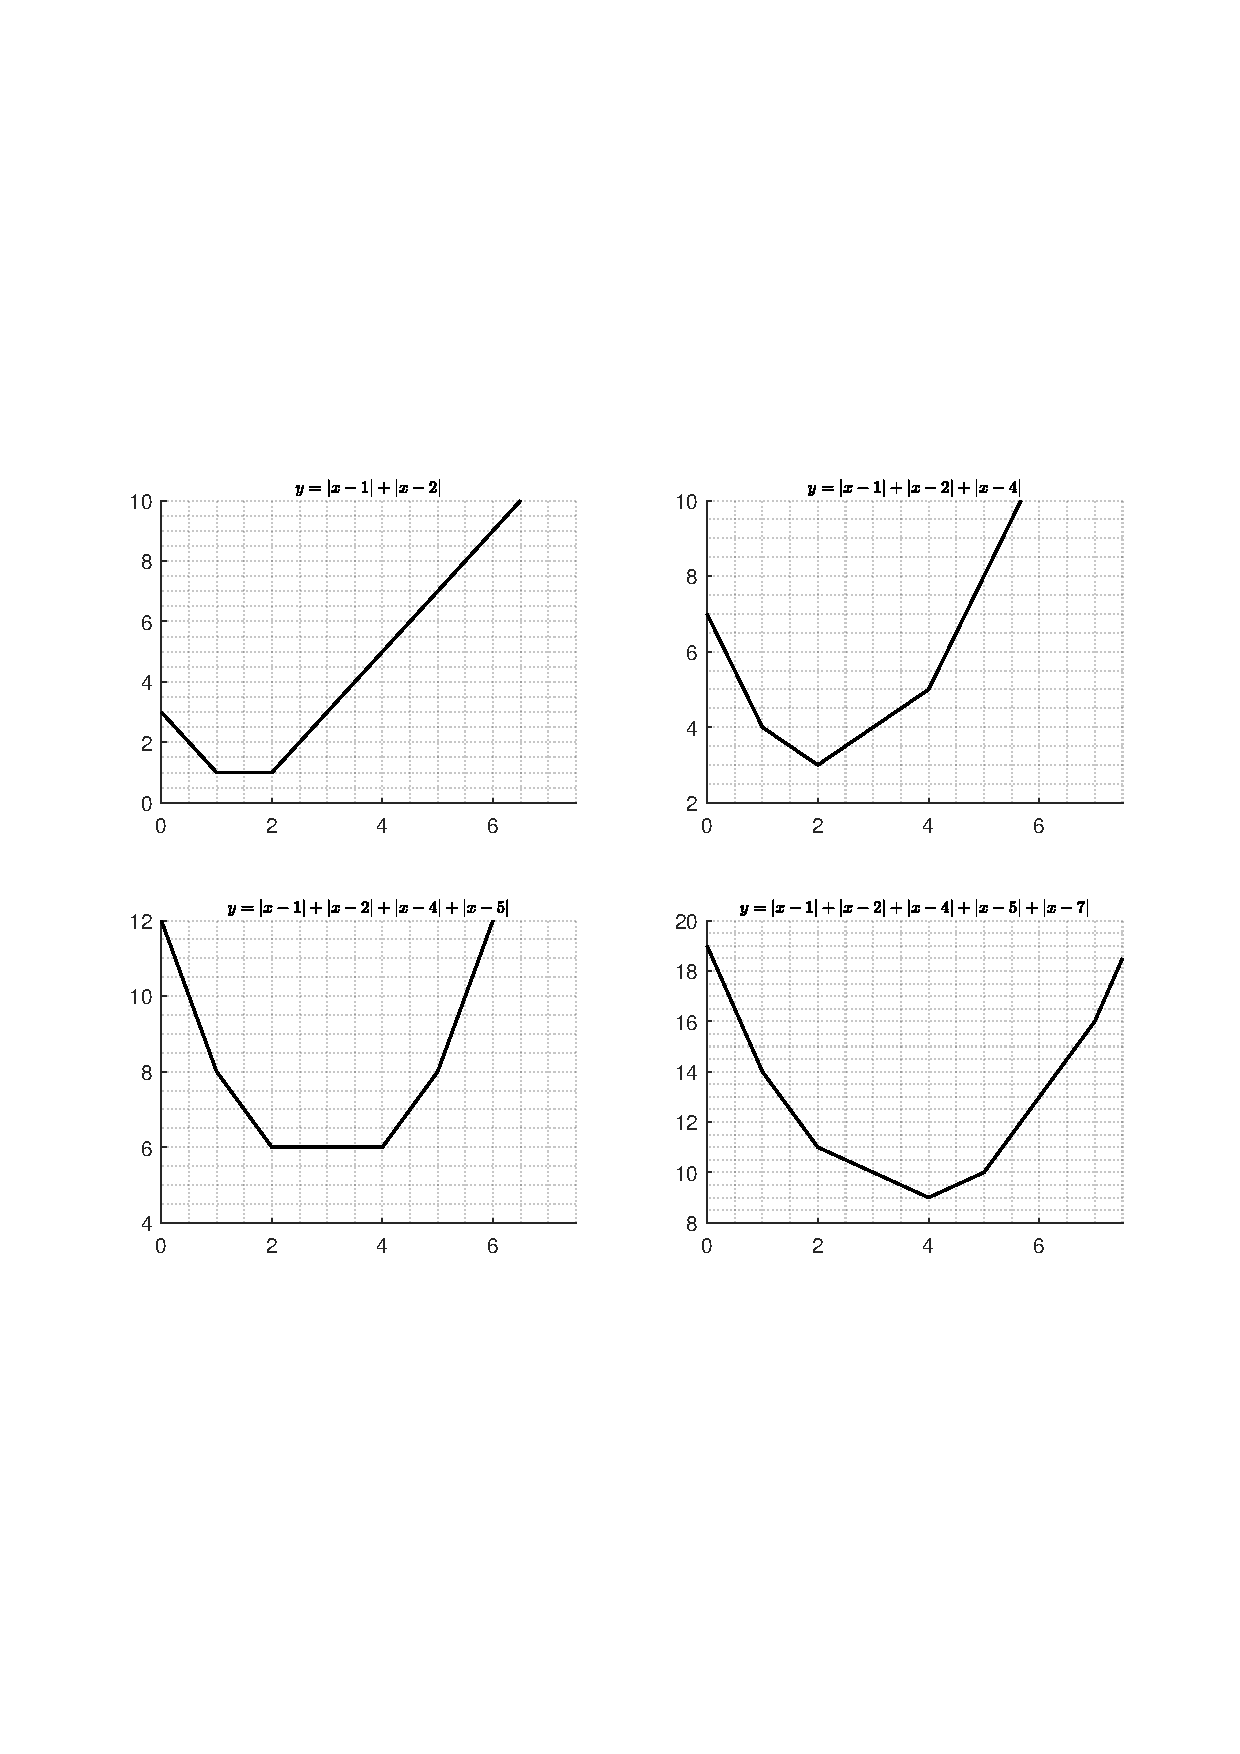
\includegraphics[width=0.8\linewidth]{多个绝对值之和}
\end{figure} 

\item 函数$ y=|x-b_1|-|x-b_2| $的图像是“两头平,中间斜”。
而$ y=|x-b_1|-|x-b_2|-|x-b_3| $的图像则比较复杂。
\begin{figure}[h]
    \centering
    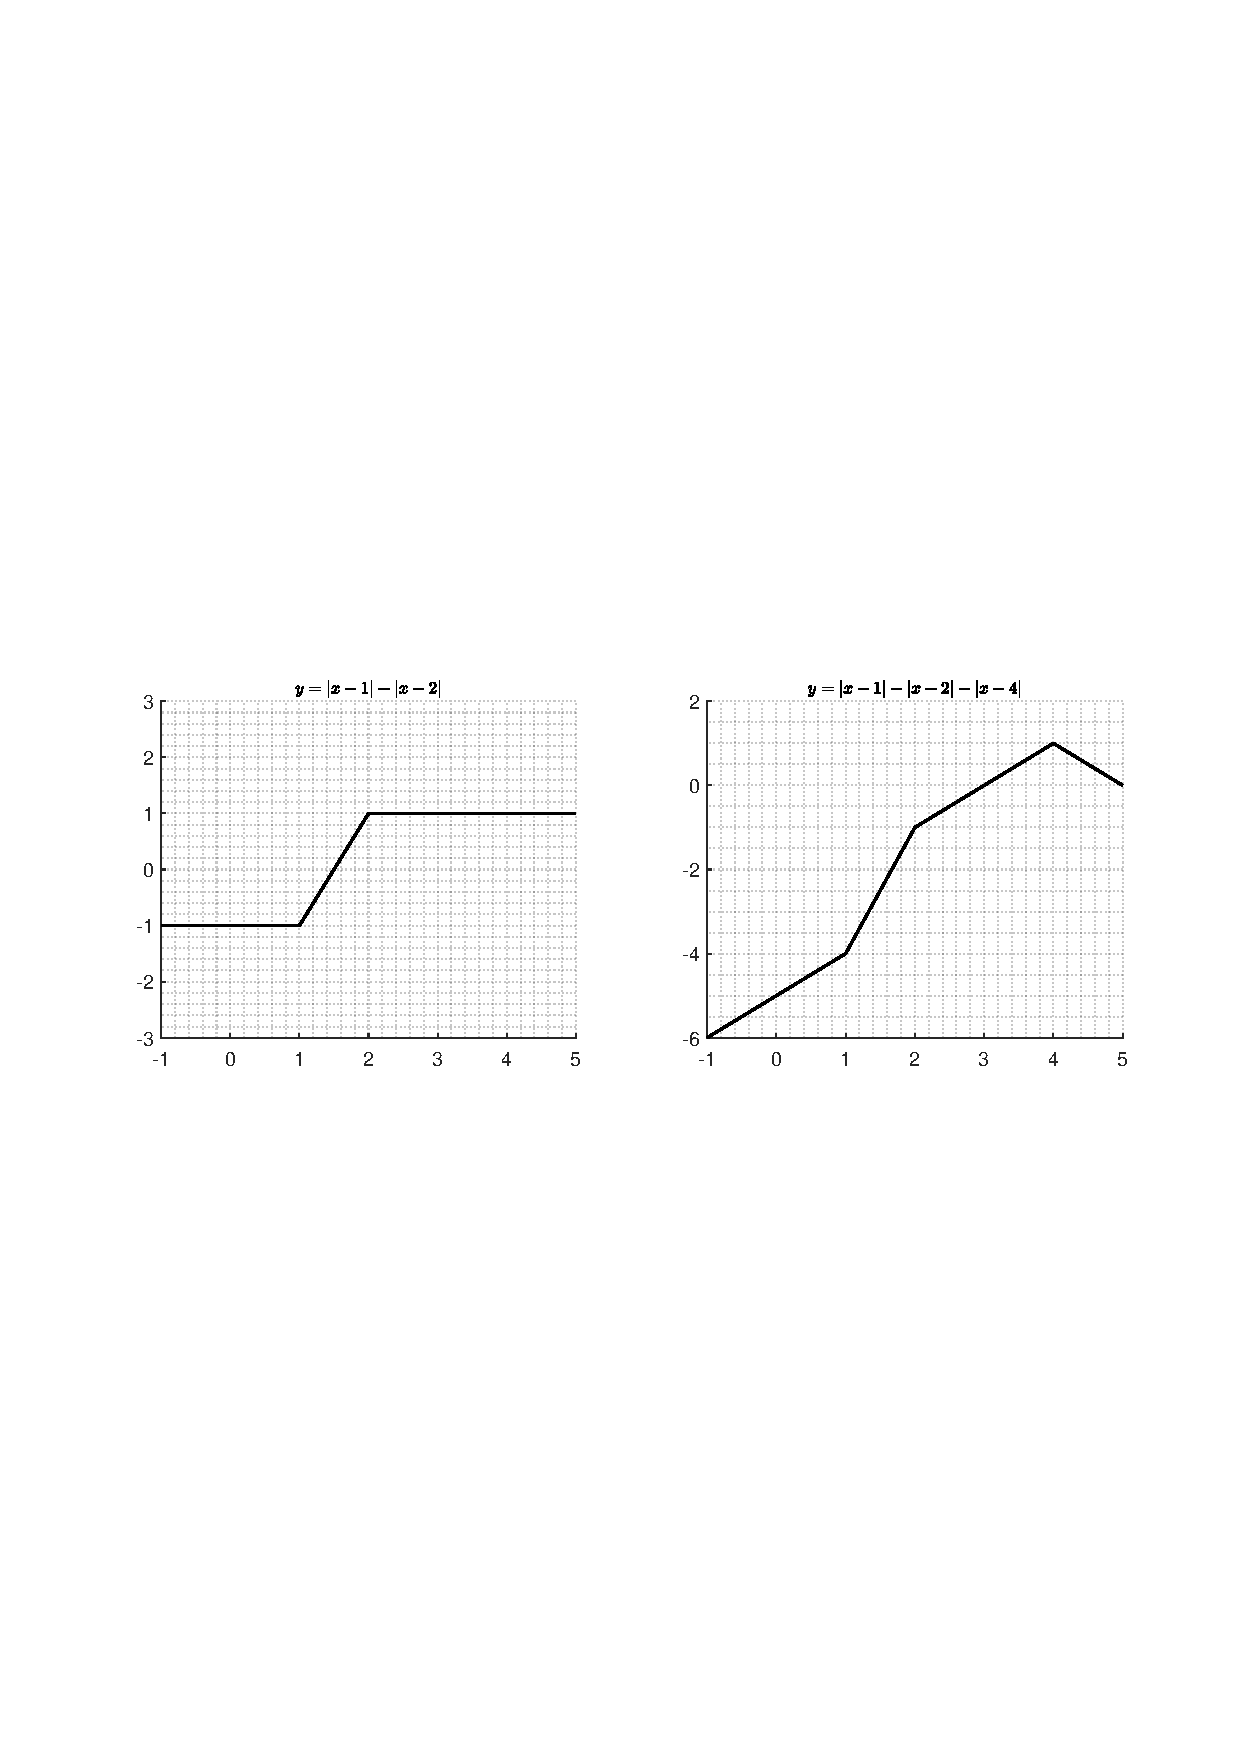
\includegraphics[width=0.8\linewidth]{几个绝对值之差}
\end{figure}

\item \textbf{零点存在定理}\ 若函数$ f(x) $在闭区间$ [a,b] $连续,
且$ f(a)\cdot f(b)<0 $,则一定存在$ x_0\in(a,b) $,使$ f(x_0)=0 $. 
此定理为二分法找函数零点的理论基础。

\item \textbf{介值定理(中间值定理)}\ 若函数$ f(x) $在闭区间$ [a,b] $连续,则它一定能取到介于最大值和最小值之间的任何一个值。

\item 解决恒成立问题或有解问题,第一步通常是分离变量,使得不等号的两侧均只包含一个变量,然后
求某一边函数的最值。($ \exists $表示存在,$ \forall $表示任意。)
\begin{align*}
    \exists\ x_0\in(a,b),\ f(x_0)>m &\ \Rightarrow \ f(x)_{\max} >m \\
    \exists\ x_0\in(a,b),\ f(x_0)<m &\ \Rightarrow \ f(x)_{\min} <m \\
    \forall\ x\in(a,b),\ f(x)<m &\ \Rightarrow \ f(x)_{\max} <m \\
    \forall\ x\in(a,b),\ f(x)>m &\ \Rightarrow \ f(x)_{\min} >m 
\end{align*}

\end{itemize}

\section{函数方程}
\begin{itemize}[leftmargin=\inteval{\myitemleftmargin}pt,itemsep=
   \inteval{\myitemitempsep}pt,topsep=\inteval{\myitemtopsep}pt]
\item 常见函数方程:
\begin{align*}
    f(x_1+x_2)=&\ f(x_1)+f(x_2)   	& f(x)=kx  \\
    f\left(\dfrac{x_1+x_2}{2}\right) =&\ \dfrac{f(x_1)+f(x_2)}{2}  & f(x)=kx+b \\
    f(x_1x_2)=&\ f(x_1)f(x_2)   	& f(x)=x^{\alpha} \\
    f(x_1+x_2)=&\ f(x_1)f(x_2)   	& f(x)=a^x \\
    f(x_1x_2)=&\ f(x_1)+f(x_2)   	& f(x)=\log_{a}x \\
    f(x_1x_2)=&\ x_2f(x_1)+x_1f(x_2)   	& f(x)=x\log_{a}x \\
    f(x_1+x_2)+f(x_1-x_2)=&\ 2\lambda f(x_1)f(x_2) & f(x)=\dfrac{1}{\lambda}\cos x \\
    f(x_1+x_2)+f(x_1-x_2)=&\ 2f(x_1)\cos x_2	& f(x)=a\cos x+b\sin x   
\end{align*}

\item 考虑$ f(x_1+x_2)=f(x_1)+f(x_2) $. \\
(1)令$ x_2=0 $,则$ f(x_1)=f(x_1)+f(0) $,所以$ f(0)=0 $. \\
(2)令$ x_2=-x_1 $,则$ f(x_1-x_1)=f(0)=f(x_1)+f(-x_1)=0 $,所以$ f(x) $是奇函数。\\
%(以上两步也适用于$ f(x_1)+f(x_2)=f\left(\dfrac{x_1+x_2}{1+x_1x_2} \right) $,
%$ \ln \dfrac{1-x}{1+x} $和$ \arctan x $满足都是奇函数。)\\
(3)任取正整数$ m,n $,有 $ f(\dfrac{m}{n})=f\Big(\dfrac{m-1}{n}+\dfrac{1}{n}\Big)=
f\Big(\dfrac{m-1}{n}\Big)+f\Big(\dfrac{1}{n}\Big)=
f\Big(\dfrac{m-2}{n}\Big)+2f\Big(\dfrac{1}{n}\Big)=
\cdots =mf\Big(\dfrac{1}{n}\Big)$,当$ m=n $时,$ f(1)=nf\Big(\dfrac{1}{n}\Big) $,
即 $ f\Big(\dfrac{1}{n}\Big)=\dfrac{1}{n}f(1) $,
所以 $f\Big(\dfrac{m}{n}\Big)=\dfrac{m}{n}f(1) $. 
如果记$ f(1)=k $,再利用$ f(x) $是奇函数的性质,那么对任意有理数$ q $,都有$ f(q)=kq $. \\
(4)对于$ x $为无理数时的情形,需要附加函数连续性的条件,并使用闭区间套定理进行分析,此处不讨论。
感兴趣的还可搜索“柯西方程的不连续解”。

\item 现在再来看小学就学过的矩形面积公式$ S=ab $,如果你觉得这是显然的、
无需证明的,那说明你缺少数学上的敏感。矩形的面积公式是基于一些更基本的
原理得出的。首先,全等的矩形,面积相等,与矩形的方向、位置无关,
长和宽对应相等的矩形是全等的
(即面积相等),所以面积$ S $只是长和宽的二元函数(长和宽分别记为$ a,b $,
不限定$ a,b $的相对大小),$ S=f(a,b)=f(b,a) $。第二,面积具有非负性,即
$ f(a,b)\geq 0 $,当$ a,b $中存在一个为0时,$ f(a,b)=0 $. 第三,
面积具有可加性,长、宽分别为$ a_1,b $和$ a_2,b $的两个矩形拼成长、宽为
$ (a_1+a_2),b $的大矩形时,后者的面积等于前两者的面积之和,即
$ f(a_1+a_2,b)=f(a_1,b)+f(a_2,b) $. 可加性也说明了$ f(a,b) $既
关于$ a $单调递增且连续,又关于$ b $单调递增且连续。
再利用上一条知识点中的方法可以得到:
对于任意非负有理数(或者非负实数)$ a,b $,有
\begin{gather*}
    f(q_1a,b)=a f(q_1,b)  \\
    f(a,q_2b)=b f(a,q_2)  \\
    f(q_1a,q_2b)=af(q_1,q_2b)=abf(q_1,q_2)
\end{gather*}
令$ q_1=q_2=1 $,有$ f(a,b)=abf(1,1) $,所以矩形面积$ S $
必须是$ ab $的常数倍,为了方便可以规定$ f(1,1)=1 $,即使规定为
其它常数也不会影响面积的本质。

\item 考虑$ f(x_1+x_2)=f(x_1)f(x_2) $,假设$ f(x) $还满足:对任意$ x\in 
\textbf{R} $,都有$ f(x)> 0 $. \\ 令$ x_2=0 $,则$ f(x_1)=f(x_1)f(0) $,所以
$ f(0)=1 $. $ f\Big(\dfrac{m}{n}\Big)=f\Big(\dfrac{m-1}{n}+\dfrac{1}{n}\Big)=
f\Big(\dfrac{m-1}{n}\Big)f\Big(\dfrac{1}{n}\Big)=f\Big(\dfrac{m-2}{n}\Big)f^2
\Big(\dfrac{1}{n}\Big)=\cdots =f^m\Big(\dfrac{1}{n}\Big) $,
当$ m=n $时,$ f(1)=f^n\Big(\dfrac{1}{n}\Big),\ f\Big(\dfrac{1}{n}\Big)
=[f(1)]^{\frac{1}{n}} $. 
所以$f\Big(\dfrac{m}{n}\Big)=f^m\Big(\dfrac{1}{n}\Big)=[f(1)]^{\frac{m}{n}} $. 

\item 考虑$ f(x_1x_2)=f(x_1)+f(x_2) $,假设$ f(x) $的定义域是$ x> 0 $. \\
令$ x_2=1 $,则$ f(x_1)=f(x_1)+f(1) $,所以$ f(1)=0 $. 
令$ x_2=\dfrac{1}{x_1} $,则$ f(1)=f(x_1x_2)=f(x_1)+f(\dfrac{1}{x_1})=0 ,
\ f\Big(\dfrac{1}{x_1}\Big)=-f(x_1) $. 又有
$ f(x^{\frac{m}{n}})=mf(x^{\frac{1}{n}}) $,
当$ m=n $时,$ f(x)=nf(x^{\frac{1}{n}}),\ f(x^{\frac{1}{n}})=\dfrac{1}{n}f(x) $. 
所以$ f(x^{\frac{m}{n}})=\dfrac{m}{n}f(x) $. 

\item $ f\left(\dfrac{x_1+x_2}{2}\right) =\dfrac{f(x_1)+f(x_2)}{2} $
可以推广成$ f\left(\lambda x_1+(1-\lambda)x_2\right) =\lambda f(x_1)+
(1-\lambda)f(x_2) $,其中$ \lambda \in (0,1) $,此时也有$ f(x)=kx+b $. 

\item 如果给以上函数方程中的函数附加上光滑可导的条件,
那还可以利用导数来分析函数的性质,比如把$ f(x_1+x_2)=
f(x_1)+f(x_2) $中的$ x_2 $先看作常数,两边对$ x_1 $求导,
可得$ f'(x_1+x_2)=f'(x_1) $,这说明$ f'(x_1) $是一个与
$ x_1 $无关的常数,即$ f'(x_1) $具有平移不变性,
那么$ f(x) $只能是直线。
%在$ f\left(\dfrac{x_1+x_2}{2}\right) =
%\dfrac{f(x_1)+f(x_2)}{2} $中,两边对$ x_1 $求导,$ \dfrac{1}{2}f'\left(\dfrac{x_1+x_2}{2}
%\right)=\dfrac{1}{2}f'(x_1) $,同样说明$ f'(x_1) $是一个与$ x_1 $无关的常数。

\item 若定义$ f(x)=\ln \dfrac{1-x}{1+x} $,则$ f(x_1)+f(x_2)=f\left(\dfrac{x_1+x_2}{1+x_1x_2} \right)  $. 
$ \ln \dfrac{1+x}{1-x},\ln \dfrac{x+1}{x-1},\ln \dfrac{x-1}{x+1}$有类似性质。另外,反正切函数也有相似形式:$ \arctan x_1+\arctan x_2=\arctan\dfrac{x_1+x_2}{1-x_1x_2} $. 

\item 满足$ f(x_1+x_2)= f(x_1)+f(x_2)+2\lambda x_1x_2 $的函数是$ f(x)=\lambda x^2+\mu x $. \\
\textbf{分析}\ 首先令$ x_2=0 $,可得$ f(x_1+0)=f(x_1)+f(0)+0 $,所以$ f(0)=0 $.
(令$ x_1=x_2=0 $也可得到$ f(0)=0 $),考虑正整数情形,
\begin{align*}
    f(2)=&\ 2f(1)+2\lambda \\
    f(3)=&\ f(2)+f(1)+4\lambda=3f(1)+6 \lambda \\
    f(4)=&\ f(3)+f(1)+6\lambda=4f(1)+12\lambda \\
    \vdots&\  
\end{align*}
用归纳法容易证明,$ f(n)=f(n-1)+f(1)+2\lambda (n-1)=nf(1)+\lambda n(n-1)=
\lambda n^2+[f(1)-\lambda]n $. 剩余步骤省略,此时已经可以大胆猜测
$ f(x)=\lambda x^2+\mu x $. 

%\item $^*$ 在数论中,满足性质$ f(x_1x_2)=f(x_1)+f(x_2) $的函数被称为“加性函数”;
%满足性质$ f(x_1x_2)=f(x_1)f(x_2) $的函数被称为“积性函数”。
%%\\
%\item 若$ A,B $代表某种试验中可能发生的两件事,而且$ A $和$ B $相互独立
%(一件事是否发生对另一件事没有影响),那么$ A,B $同时发生的概率等于两者各自发生
%的概率之积(具有积性),
%即$ P(AB)=P(A)P(B) $,有些书上也写成$ P(A\cap B)=P(A)P(B) $. 
%\newpage

\end{itemize}

\section{函数迭代}
\begin{itemize}[leftmargin=\inteval{\myitemleftmargin}pt,itemsep=
   \inteval{\myitemitempsep}pt,topsep=\inteval{\myitemtopsep}pt]
\item 同一个函数$ f(x) $不断地复合,
$ f(f(x)),f(f(f(x))) \cdots $称为函数的迭代。
记$ f_0(x)=x,\ f_1(x)=f(x),\ f_{n+1}(x)=f(f_n(x)) $. 
则$ f_n(x) $称为函数$ f(x) $的$ n $次迭代。一些函数迭代如表\ref{函数迭代列表}
\footnote{张伟年. 动力系统基础[M]. 高等教育出版社,施普林格出版社, 2001.}:
\begin{table}[h] 
\centering
\renewcommand\arraystretch{1.5}  
\caption{}   
\begin{tabular}{|c|c|} 
    \hline
    $ f(x) $ & $ f_n(x) $ \\
    \hline
    $ x+2\sqrt{x}+1 $ & $ (\sqrt{x}+n)^2 $ \\
    \hline
    $ \dfrac{x}{a+bx} $ & $ \dfrac{x}{a^n+\dfrac{1-a^n}{1-a}bx} $ \\
    \hline
    $ \sqrt[k]{ax^k+b} $ & $ \sqrt[k]{a^nx^k+\dfrac{1-a^n}{1-a}b} $ \\
    \hline
    $ x^2+2x $ & $ (x+1)^{2^n}-1 $ \\
    \hline
    $ \dfrac{x^2}{2x-1} $ & $\dfrac{x^{2^n}}{x^{2^n}-(x-1)^{2^n}}$ \\
    \hline
    $ \dfrac{x}{\sqrt[k]{1+ax^k}} $ & $ \dfrac{x}{\sqrt[k]{1+nax^k}}  $ \\
    \hline
    $ \dfrac{x}{1+2a\sqrt{x}+a^2x} $ & $ \dfrac{x}{(1+na\sqrt{x})^2} $ \\
    \hline
    $ 2x\sqrt{1-x^2} $ & $ \sin(2^n\cdot \arcsin x) $ \\
    \hline
    $ 2x^2-1 $ & $ \cos(2^n\cdot \arccos x) $ \\
    \hline
    $ \dfrac{2x}{1-x^2} $ & $ \tan(2^n\cdot \arctan x) $ \\
    \hline
\end{tabular}
%\vspace{-3mm}
\label{函数迭代列表}
\end{table} 

表中最后3个函数只需看成三角函数的二倍角公式,即$ 2\sin \theta\cos \theta $,
$ 2\cos^2 \theta-1 $,$ \dfrac{2\tan \theta}{1-\tan^2 \theta} $. 
表中的结果用数学归纳法是容易证明的。

\item 函数的迭代也可看成数列的递推,有些数列是周期数列,
有些函数迭代也会有周期。如果存在自然数$ T $,
满足$ f_{n+T}(x)=f_n(x) $,则$ T $称为$ f(x) $
的迭代周期,$ f_{n+T}(x)=f_n(x) $等价于$ f_T(x)=f_0(x)=x $. 
比如$ f(x)=\sqrt[3]{\dfrac{x^3-1}{x^3+1}} $的迭代周期是4.
$ f(x)=\dfrac{(\cos \dfrac{2\pi}{n})x-\sin \dfrac{2\pi}{n}}
{(\sin\dfrac{2\pi}{n})x+\cos \dfrac{2\pi}{n}} $的迭代周期是$ n $. 


\end{itemize}

\section{多项式}
\begin{itemize}[leftmargin=\inteval{\myitemleftmargin}pt,itemsep=
   \inteval{\myitemitempsep}pt,topsep=\inteval{\myitemtopsep}pt]
\item 三次函数$ y=ax^3+bx^2+cx+d $也是一种三次曲线,
通过平移变换$ x=t-\dfrac{b}{3a} $,可以消去三次函数的二次项,
如果再做上下平移消去常数项,就可得到一个奇函数(关于原点中心对称),说明任意三次函数的图像都是中心对称图形,对称中心坐标为 $ (-\dfrac{b}{3a},f(-\dfrac{b}{3a})) $. 

\item 三次方程韦达定理:$ x^3+\dfrac{b}{a}x^2+\dfrac{c}{a}x+
\dfrac{d}{a}=(x-x_1)(x-x_2)(x-x_3)=0$,则
\begin{align}\label{三次方程韦达定理}
    x_1+x_2+x_3=-\dfrac{b}{a},\ x_1x_2+x_1x_3+x_2x_3=\dfrac{c}{a},\ x_1x_2x_3=-\dfrac{d}{a}
\end{align}
可以从量纲的角度来进行理解和记忆,假设$ x $代表长度,那么$ x^3 $就代表体积,
因为只有单位相同的物理量才能相加减,所以$ \dfrac{b}{a} $代表长度,$ \dfrac{c}{a} $代表面积,
$ \dfrac{d}{a} $代表体积。而$ x_1+x_2+x_3 $代表长度,$ x_1x_2+x_1x_3+x_2x_3 $代表面积,
$ x_1x_2x_3 $代表体积。单位相同的物理量才能相等。

请读者思考一般的$ n $次方程的韦达定理。

\item 三次不等式的解集。假设$ x_1<x_2<x_3 $,那么$ f(x)=(x-x_1)(x-x_2)(x-x_3)
<0 $的解集为$ (-\infty,x_1)\cup (x_2,x_3) $;$ f(x)>0 $的解集为$ (x_1,x_2)\cup
(x_3,+\infty) $. 

\item 由(\ref{三次方程韦达定理})式可得:
\begin{align*}
     &\ x_1^2x_2^2+x_1^2x_3^2+x_2^2x_3^2 \\ 
    =&\  (x_1x_2+x_1x_3+x_2x_3)^2- 2x_1x_2x_3(x_1+x_2+x_3)\\
    =&\  \dfrac{c^2-2bd}{a^2} \\
     &\ x_1^2+x_2^2+x_3^2 \\
    =&\ (x_1+x_2+x_3)^2-2(x_1x_2+x_1x_3+x_2x_3) \\
    =&\ \dfrac{b^2-2ac}{a^2} \\
     &\ (x_1-x_2)^2+(x_1-x_3)^2+(x_2-x_3)^2 \\
    =&\  2[x_1^2+x_2^2+x_3^2-(x_1x_2+x_1x_3 +x_2x_3)]\\ 
    =&\  2[(x_1+x_2+x_3)^2-3(x_1x_2+x_1x_3+x_2x_3)] \\
    =&\  \dfrac{2(b^2-3ac)}{a^2}
\end{align*}
以上等式说明,如果$ x_1,x_2,x_3 $均为实数,那么必有$ c^2-2bd\geq 0,\ b^2-2ac \geq 0,\ 
b^2-3ac \geq 0 $. \\
%令$ s_k=x_1^k+x_2^k+\cdots+ x_n^k(k\geq 1);s_0=n.$
%\begin{align*}
%	&\sigma_1=x_1+x_2+\cdots+x_n \\
%	&\sigma_2=x_1x_2+x_1x_3\cdots+x_{n-1}x_n=\sum_{1\leq i<j\leq n}x_ix_j \\
%	&\cdots \\
%	&\sigma_n=x_1x_2\cdots x_n		
%\end{align*}
%
%牛顿公式:
%\begin{align*}
%	k< n ,\  &s_k-s_{k-1}\sigma_1+s_{k-2}\sigma_2-\cdots 
%+(-1)^{k-1}s_1\sigma_{k-1}+(-1)^kk\sigma_k=0 \\
%	k\geq n ,\  &s_k-s_{k-1}\sigma_1+s_{k-2}\sigma_2-\cdots+(-1)^ns_{k-n}\sigma_n=0 
%\end{align*} 

\item 常用因式分解:
\begin{align*}
    &  a^3-b^3=(a-b)(a^2+ab+b^2) \\
    &  a^3+b^3=(a+b)(a^2-ab+b^2) \\
    &  a^4-b^4=(a-b)(a^3+a^2b+ab^2+b^3)=(a^2-b^2)(a^2+b^2)=(a-b)(a+b)(a^2+b^2) \\
    &  a^3+b^3+c^3-3abc=(a+b+c)(a^2+b^2+c^2-ab-bc-ca) \\
    =&\ (a+b+c)\cdot \dfrac{1}{2}\left[(a^2+b^2-2ab)
    +(b^2+c^2-2bc)+(c^2+a^2-2ca) \right]
\end{align*}
\item 如果$ a,b,c $均为非负数,那么$ a^3+b^3+c^3 \geq 3abc $,把$ a,b,c $分别换成
$ \sqrt[3]{a},\sqrt[3]{b},\sqrt[3]{c} $,有$ a+b+c \geq 3 \sqrt[3]{abc}$. 

\item 因式分解练习:
\begin{align*}
    &  2x^3+3x^2-1=(2x^3+2x^2)+(x^2-1)=2x^2(x+1)+(x-1)(x+1)=(2x-1)(x+1)^2 \\
    &  2x^3-3x^2+1=(2x^3-2x^2)-(x^2-1)=2x^2(x-1)-(x-1)(x+1)=(2x+1)(x-1)^2 \\
    &  x^3-2x+1=x(x^2-1)-(x-1)=(x^2+x-1)(x-1) \\
    &  x^3-2x-1=x(x^2-1)-(x+1)=(x^2-x-1)(x+1) \\
    &  x^3+2x^2-2x-1=(x-1)(x^2+3x+1)
    %&a^3-2a^2-5a+6=(a-1)(a+2)(a-3)\\
    %&2a^3-a^2-5a-2=(a+1)(2a+1)(a-2)\\
    %&3a^4-4a^3-57a^2-14a+120=(a+2)(a+3)(3a-4)(a-5)\\
    %&5a^3+7a^2b-15a^2+2ab^2-21ab-6b^2=(a+b)(5a+2b)(a-3)\\
    %&2a^4-7a^3b+a^2b^2+7ab^3-3b^4=(a+b)(a-b)(a-3b)(2a-b)\\
    %&18a^4+39a^3b+23a^2b^2+ab^3-b^4=(a+b)^2(6a-b)(3a+b)
\end{align*}

\end{itemize}

\section{凹凸性}
\begin{itemize}[leftmargin=\inteval{\myitemleftmargin}pt,itemsep=
   \inteval{\myitemitempsep}pt,topsep=\inteval{\myitemtopsep}pt]

% HanShuAoTuXing.m
\item 函数的凹凸性是指$ \dfrac{f(x_1)+f(x_2)}{2} $与
$ f(\dfrac{x_1+x_2}{2}) $的相对大小,本小节均默认$ x_1 \neq x_2 $. 
更一般地,是比较$ \lambda f(x_1)+(1-\lambda)f(x_2) $ 
与$ f(\lambda x_1+(1-\lambda)x_2) $的大小,其中$ \lambda \in (0,1) $. 
函数的凹凸性直接由二阶导数的正负决定。因为不同的书上对凹函数与凸函数的定义
已经完全混乱,所以本书也不具体定义什么是凹、什么是凸,统称为凹凸性。
\begin{figure}[H]
    \centering
    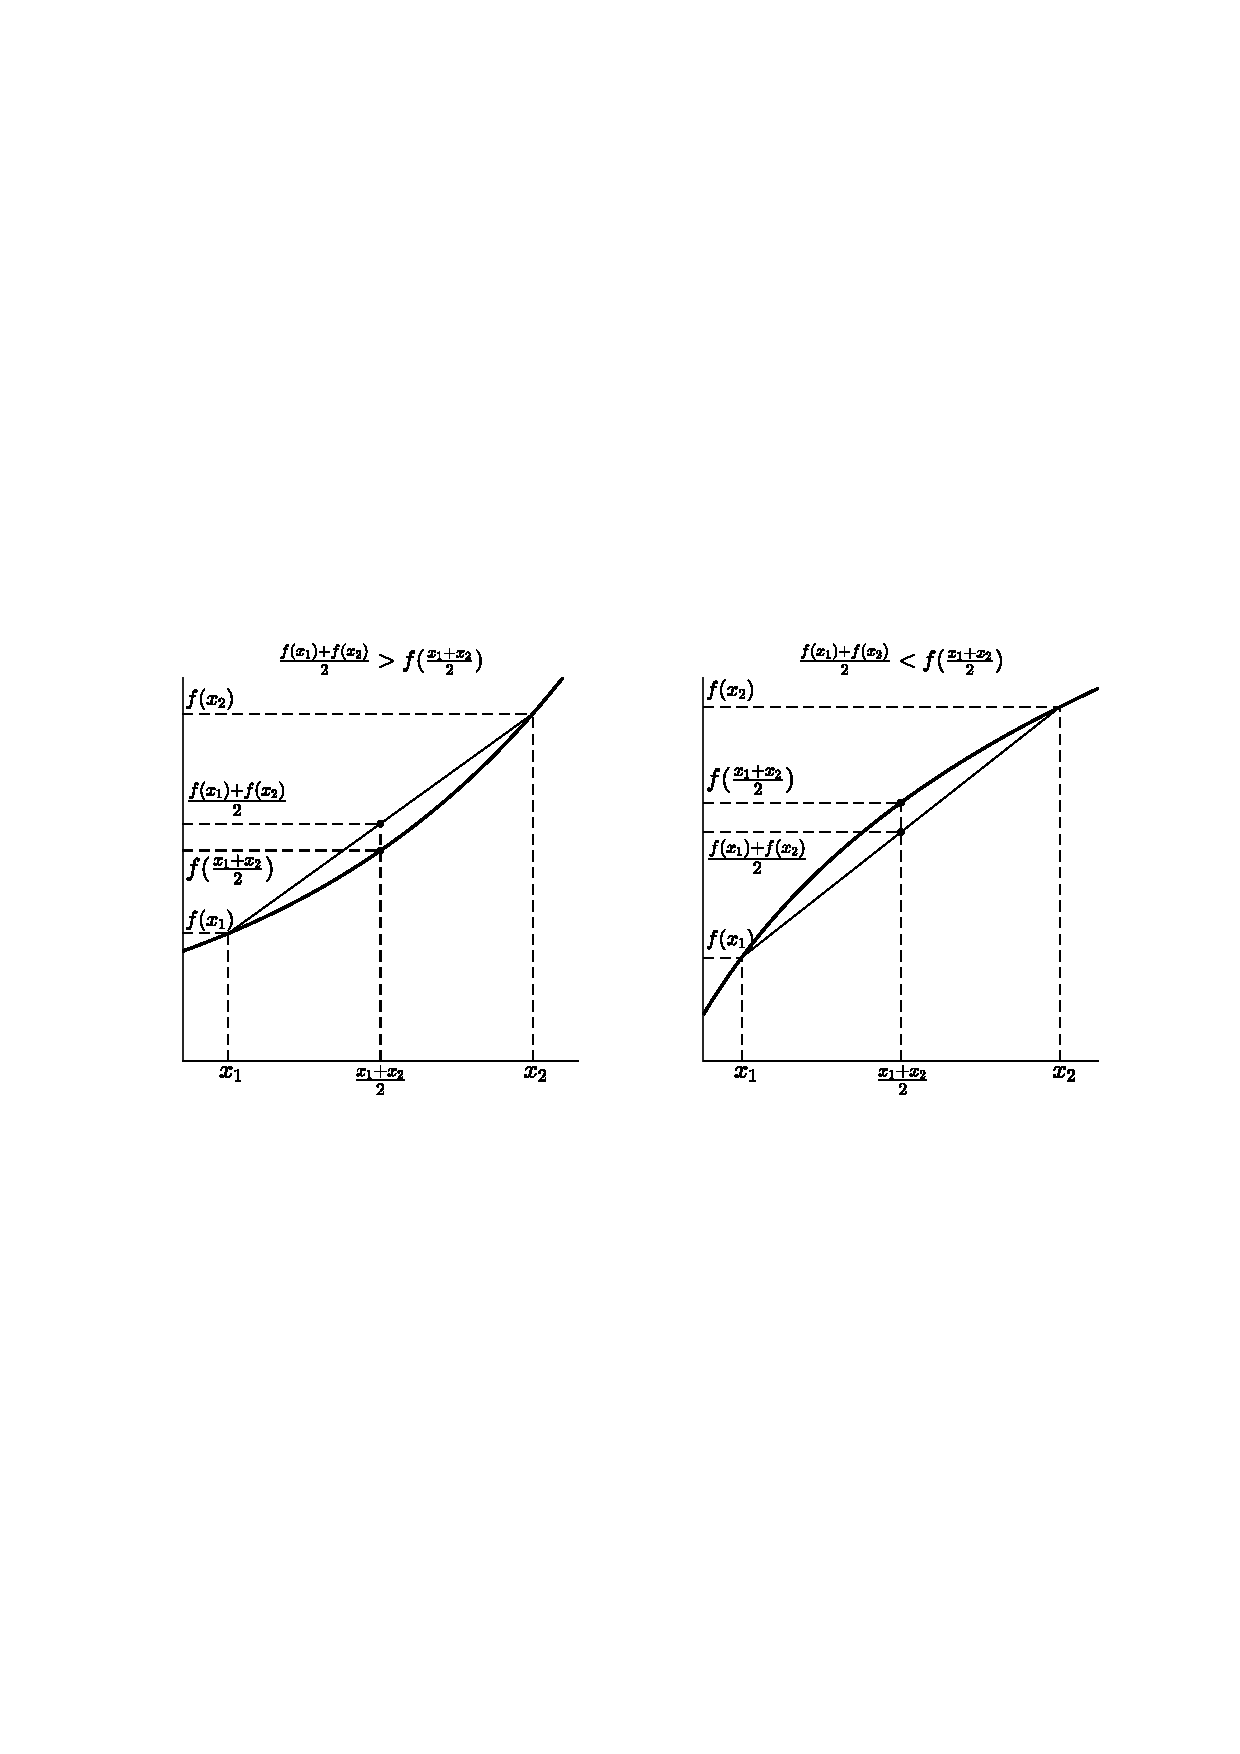
\includegraphics[width=0.8\linewidth]{函数凹凸性主图}
\end{figure}

\noindent \textbf{三角函数} \\
当$ x_1,x_2\in (0,\pi) $时,
\begin{align*}
    \dfrac{1}{2} \left(\sin x_1 + \sin x_2 \right) =&\ 
    \dfrac{1}{2} \left[ \sin \left(\dfrac{x_1+x_2}{2}+\dfrac{x_1-x_2}{2}\right)  + 
    \sin \left(\dfrac{x_1+x_2}{2}-\dfrac{x_1-x_2}{2}\right) \right] \\
    =&\  \sin \dfrac{x_1+x_2}{2} \cos \dfrac{x_1-x_2}{2} 
     < \sin \dfrac{x_1+x_2}{2}
\end{align*}
当$ x_1,x_2\in (0,\dfrac{\pi}{2}) $时,
\begin{align*}
    \dfrac{1}{2}\left(\tan x_1+\tan x_2\right)-\tan\dfrac{x_1+x_2}{2}
    =&\  \dfrac{\sin\dfrac{x_1+x_2}{2}\left(\cos^2\dfrac{x_1+x_2}{2}
        -\cos x_1\cos x_2 \right)}{\cos x_1\cos x_2 \cos\dfrac{x_1+x_2}{2}}\\
    =&\  \dfrac{\sin\dfrac{x_1+x_2}{2}\left[1-\cos(x_1-x_2) \right]}
    {2\cos x_1\cos x_2 \cos\dfrac{x_1+x_2}{2}} >0
\end{align*}
\\
\textbf{指数函数和对数函数} \\
\begin{align*}
    \dfrac{\e^{x_1}+\e^{x_2}}{2}>\sqrt{\e^{x_1}·\e^{x_2}}=\e^{\frac{x_1+x_2}{2}}
\end{align*}
\begin{align*}
    \dfrac{\ln x_1+\ln x_2}{2}=\ln \sqrt{x_1 x_2}<\ln\dfrac{x_1+x_2}{2}
\end{align*}
$ \e^x $与$ \ln x $互为反函数,两者的图像关于直线$ y=x $对称,请结合图像思考上面两个不等式的含义。\\
\\
\textbf{幂函数} \\
若$ \alpha $为实数,$ 0<x_1<x_2 $,
\begin{align*}
    \dfrac{x_1^{\alpha}+x_2^{\alpha}}{2}-\left( \dfrac{x_1+x_2}{2}\right)^{\alpha} =&\ 
    x_1^{\alpha}\left[\frac{1+\left( \frac{x_2}{x_1}\right)^{\alpha} }{2}-
    \left(\frac{1+\frac{x_2}{x_1}}{2} \right)^{\alpha} \right]   \\
    =&\  x_1^{\alpha}\left[ \dfrac{1+t^{\alpha}}{2}-\left(\dfrac{1+t}{2} 
    \right)^{\alpha}  \right]  =x_1^{\alpha}f(t)
\end{align*}
其中,$ t=\dfrac{x_2}{x_1}>1 $,
\begin{align*}
    f'(t)=\dfrac{\alpha}{2}\left[ t^{\alpha-1}-
    \left( \dfrac{1+t}{2}\right)^{\alpha-1}\right]
\end{align*}
$ f(1)=0,f'(1)=0 $,当$ t>1 $时,若$ \alpha>1 $或$ \alpha<0 $,
则$ f'(t)>0 $,$ f(t)>f(1)=0 $. 
若$ 0<\alpha<1 $,则$ f(t)<0 $. 
例如,$ \dfrac{x_1^2+x_2^2}{2}>\left(\dfrac{x_1+x_2}{2}\right)^2,\  \dfrac{\sqrt{x_1}+\sqrt{x_2}}{2}<\sqrt{\dfrac{x_1+x_2}{2}} $.  

\item 若$ \alpha $为大于1的正整数(记为$ n $),还可用其它方法证明
\begin{gather}\label{幂函数凹凸性不等式}
    \dfrac{x_1^n+x_2^n}{2}>\left( \dfrac{x_1+x_2}{2}\right)^n
\end{gather}
\textbf{方法一}\ 二项式定理。设$ 0<k<n $,则$ (x_2^k-x_1^k)(x_2^{n-k}-x_1^{n-k})=x_2^n+x_1^n-x_2^kx_1^{n-k}-x_1^kx_2^{n-k}>0 $,故
$ x_2^n+x_1^n > x_2^kx_1^{n-k}+x_1^kx_2^{n-k} $,于是:
\begin{align*}
    2^n(x_1^n+x_2^n)-& 2(x_1+x_2)^n \\
    =2^n(x_1^n+x_2^n)-&\bigl[C_n^0(x_1^n+x_2^n)+C_n^1(x_1^{n-1}x_2+x_2^{n-1}x_1)+\cdots\\
    + &\ C_n^{n-1}(x_1x_2^{n-1}+x_2x_1^{n-1})+C_n^n(x_2^n+x_1^n) \bigr] \\
    >2^n(x_1^n+x_2^n)-&\bigl[C_n^0(x_1^n+x_2^n)+C_n^1(x_1^n+x_2^n)
    +\cdots \\+ &C_n^{n-1}(x_1^n+x_2^n)+C_n^n(x_2^n+x_1^n) \bigr] \\
    =2^n(x_1^n+x_2^n)-&(C_n^0+C_n^1+\cdots +C_n^{n-1}+C_n^n)(x_1^n+x_2^n) = 0
\end{align*}
\textbf{方法二}\ 数学归纳法。因为 $ (x_1^n-x_2^n)(x_1-x_2)>0 $,所以
$ x_1^nx_2+x_1x_2^n<x_1^{n+1}+x_2^{n+1} $,于是
\begin{align*}
    \left(\dfrac{x_1+x_2}{2} \right)^{n+1} =
    \left(\dfrac{x_1+x_2}{2} \right)^{n}\cdot \dfrac{x_1+x_2}{2}
    <\dfrac{x_1^n+x_2^n}{2}\cdot
    \dfrac{x_1+x_2}{2} <\dfrac{x_1^{n+1}+x_2^{n+1}}{2} 
\end{align*}


\end{itemize}

\section{例题} 

\begin{enumerate}[label={【\textbf{例\thechapter.\arabic*}】},
 leftmargin=\inteval{\myenumleftmargin}pt,
 itemsep=\inteval{\myenumitempsep}pt,
 itemindent=\inteval{\myenumitemindent}pt]
 
\item \label{用二分法预测比赛结果进行诈骗}
假如你在某一年的世界杯赛事之前,收到了来自陌生人的短信,
短信中声称他们构建了先进的数学模型,能预测足球比赛的结果,
并预测下一场小组赛中甲队将战胜乙队,比完以后发现预测正确。
接下来的若干场比赛之前,你都收到了预测比赛结果的短信,
而且全部预测正确。在总决赛之前,你还是收到了短信,说:“
我们已经预测出了冠军是谁,你只要支付100元,就能知道预测结果,
然后去买竞猜型足球彩票获得巨额收益”。那你是否要相信
他们的预测能力并支付100元呢? \\
\textbf{解}\ 答案当然是否定的,之所以能保证前面的预测全部正确,是因为诈骗
者采用了二分法。从一开始就选择足够庞大的人群,对一半的人
预测甲队获胜,对另一半的人预测乙队获胜。下次群发预测短信,
则只发给上次收到了正确预测结果的人,如此重复下去,
总有一些人收到的预测结果全部正确,在此基础上骗人交钱,
成功率就高多了。\\
同样的诈骗手段也经常被用于预测股票、期货、数字货币
等投资产品的涨跌上,诈骗者创建大量的聊天群,
在一半的聊天群中预测某股票会涨,在另一半的聊天群中预测该股票会跌,
下一次的预测只面向上次预测正确的群体。经过若干次正确预测后,
引诱他人付费购买预测结果的成功率便能大大提升。

\item Dirichlet(狄利克雷)函数:$ D(x)=
\begin{cases}
    1,\ x\text{为有理数} \\
    0,\ x\text{为无理数} \\
\end{cases} $. \\
它是偶函数,值域为$ \{0,1\} $,无法绘制函数图像,任何正有理数都是它的周期,但无最小正周期。2012年福建高考理科数学选择题第7题考了此函数。

\item 设$ f(x)=x^2+bx+c $,求证:$ |f(1)|,|f(2)|,|f(3)| $中至少有一个不小于
$ \dfrac{1}{2} $. \\
\textbf{证}\ 用反证法,假设$ |f(1)|,|f(2)|,|f(3)| $均小于$ \dfrac{1}{2} $,
$ \begin{cases}
 f(1)=1+b+c \\
 f(2)=4+2b+c \\
 f(3)=9+3b+c 
\end{cases} $,
于是有$ f(1)+f(3)-2f(2)=2 $,那么
\begin{gather*}
 2=|f(1)+f(3)-2f(2)|\leq |f(1)|+|f(3)|+2|f(2)|<
 \dfrac{1}{2}+\dfrac{1}{2}+2\cdot \dfrac{1}{2}=2
\end{gather*}
这就产生了矛盾,所以假设不成立。

为什么$  f(1)+f(3)-2f(2) $恰好等于2呢?实际上是用待定系数法确定的系数,
\begin{align*}
 \lambda_1 f(1)+\lambda_2 f(2)+\lambda_3 f(3)=&\ \lambda_1 (1+b+c)+
 \lambda_2 (4+2b+c)+\lambda_3 (9+3b+c)  \\
 =&\ (\lambda_1+4\lambda_2+9\lambda_3)+
 (\lambda_1+2 \lambda_2+ 3\lambda_3)b+(\lambda_1+\lambda_2+\lambda_3)c
\end{align*}
为使该式不包含$ b,c $,
那么$ \begin{cases}
 \lambda_1+2 \lambda_2+ 3\lambda_3=0 \\
 \lambda_1+\lambda_2+\lambda_3=0
\end{cases} $,
解得$ \lambda_2=-2 \lambda_1,\ \lambda_3=\lambda_1 $. 
于是$ \lambda_1+4\lambda_2+9\lambda_3=2\lambda_1.\ \lambda_1$可取任意非零值。

\item (2022,浙江高考)已知$a,b\in\mathbf{R}$,若对任意$x\in\mathbf{R} $, 
$ a|x-b|+|x-4|-|2x-5|\geq 0$,则(\q ) \\
A.$a\leq 1,b\geq 3$\qquad   B.$a\leq 1,b\leq 3$ \qquad
C.$a\geq 1,b\geq 3$\qquad   D.$a\geq 1,b\leq 3$ \\
\textbf{解}\ 选D. 令$x\to+\infty $,
\begin{gather*}
    ax-ab+x-4-2x+5\geq 0 \\
    (a-1)x\geq ab-1\ (\text{常数}) \\
    a\geq 1
\end{gather*}
令$ x=b $,
\begin{gather*}
    |b-4| \geq |2b-5| \\
    (b-4)^{2}-(2b-5)^{2}\geq 0 \\
    -3(b-3)(b-1)\geq 0 \\
    1 \leq b\leq 3
\end{gather*}

\item 定义在\textbf{R}上的奇函数$ f(x) $满足$ f(x)=f(a-x) $,其中$ a \neq 0 $,求$ f(x) 
$的周期。\\
\textbf{解}\ $ f(x)=f(a-x)=-f(x-a)=-f(a-(x-a))=-f(2a-x)=f(x-2a) $,
所以$ f(x) $的周期为$ 2a $. 另外,
$ f(x+\dfrac{a}{2})=f(a-(x+\dfrac{a}{2}))=f(\dfrac{a}{2}-x) $,
说明$ x=\dfrac{a}{2} $是$ f(x) $的一条对称轴。\\
\textbf{推广1}:如果$ f(x) $满足$ f(x+a)=f(b-x) $,用$ x-a $换其中的$ x $,则有$ f(x)=f(a+b-x) $,
那么$ x=\dfrac{a+b}{2} $是$ f(x) $的一条对称轴。\\
\textbf{推广2}:如果$ f(x) $同时具有对称轴和对称中心,且对称轴和对称中心的横坐标不相同,
那么$ f(x) $是周期函数。\\
\textbf{证}\ 设$ f(x) $的对称轴是$ x=a $,对称中心是$ (b,c) $,
且$ a\neq b $,那么
\begin{gather}
    f(a-x)=f(a+x) \label{fx对称轴} \\
    f(b-x)+f(b+x)=2c \label{fx对称中心}
\end{gather}
把(\ref{fx对称轴})式中的$ x $换成$ b-x $,(\ref{fx对称中心})式中的$ x $
换成$ a-x $,有
\begin{gather*}
    f(a-b+x)=f(a+b-x)  \\
    f(b-a+x)+f(b+a-x)=2c \
\end{gather*}
由以上两式消去$ f(a+b-x) $可得:
\begin{align*}
    f(b-a+x)+f(a-b+x)=&\ 2c \\
    f(x)+f(2a-2b+x) =&\ 2c \quad (\text{上式中的$ x $换成$ x+a-b $})\\
    f(2a-2b+x)+f(4a-4b+x)=&\ 2c \quad(\text{上式中的$ x $换成$ x+2a-2b $})
\end{align*}
于是$ f(x)=f(4a-4b+x) $,$ f(x) $的周期是$ 4|a-b| $. 

\item 若$ f(x) $满足$ f(x)=\pm\dfrac{1}{f(x+a)} $,那么$ f(x+2a)=\pm
\dfrac{1}{f(x+a)}=f(x) $,$ 2a $是$ f(x) $的一个周期。

\item $ f(x)=x\left( \dfrac{1}{\e^x-1}+\dfrac{1}{2}\right),
\ g(x)=\dfrac{\e^x}{\e^x+1}-\dfrac{1}{2}  $,
证明:$ f(x) $为偶函数,$ g(x) $为奇函数。\\
\textbf{证}\ 
\begin{gather*}
f(x)=\dfrac{x(\e^x+1)}{2(\e^x-1)}=\dfrac{x(1+\e^{-x})}{2(1-\e^{-x})}
=\dfrac{(-x)(\e^{-x}+1)}{2(\e^{-x}-1)}=f(-x) \\
g(x)=\dfrac{\e^x-1}{2(\e^x+1)}=\dfrac{1-\e^{-x}}{2(1+\e^{-x})}=-g(-x)
\end{gather*}

如果把$ \e^x $换成$ a^x $,并不会影响$ f(x),g(x) $的奇偶性。\\
\textbf{注}$ ^* $ $ \dfrac{x}{\e^x-1} $为伯努利数$ B_n $的生成函数,
\begin{gather*}
    \dfrac{x}{\e^x-1}=\sum\limits_{n=0}^{\infty}B_n\dfrac{x^n}{n!} 
\end{gather*}
可参看《 特殊函数概论》\footnote{
    王竹溪,郭敦仁. 特殊函数概论[M].北京大学出版社, 2012.7,第1页。}。

$ g(x)+\dfrac{1}{2}=\dfrac{\e^x}{\e^x+1}=\dfrac{1}{1+\e^{-x}}
\in (0,1) $被称为Sigmoid函数,令$ y=\dfrac{1}{1+\e^{-x}} $,则
Sigmoid函数满足微分方程$ y'=y(1-y) $,同时,
\begin{gather*}
    0<y'=y(1-y)=\dfrac{1}{1+\e^{-x}}\cdot\dfrac{1}{1+\e^{x}}
    =\dfrac{1}{2+\e^{x}+\e^{-x}}\leq\dfrac{1}{4}
\end{gather*}
$ \dfrac{\e^x}{\e^x+1},\ \dfrac{x\e^x}{\e^x+1},\ \ln\left(\dfrac{\e^x}{\e^x+1}\right),
 \tanh(x)=\dfrac{\e^x-\e^{-x}}{\e^x+\e^{-x}},\ \dfrac{x}{1+|x|},\ 
\ln(\e^x+1) $都是人工神经网络中常用的函数,图像如下。
\begin{figure}[!htbp]   % AI_Function.m
    \centering
    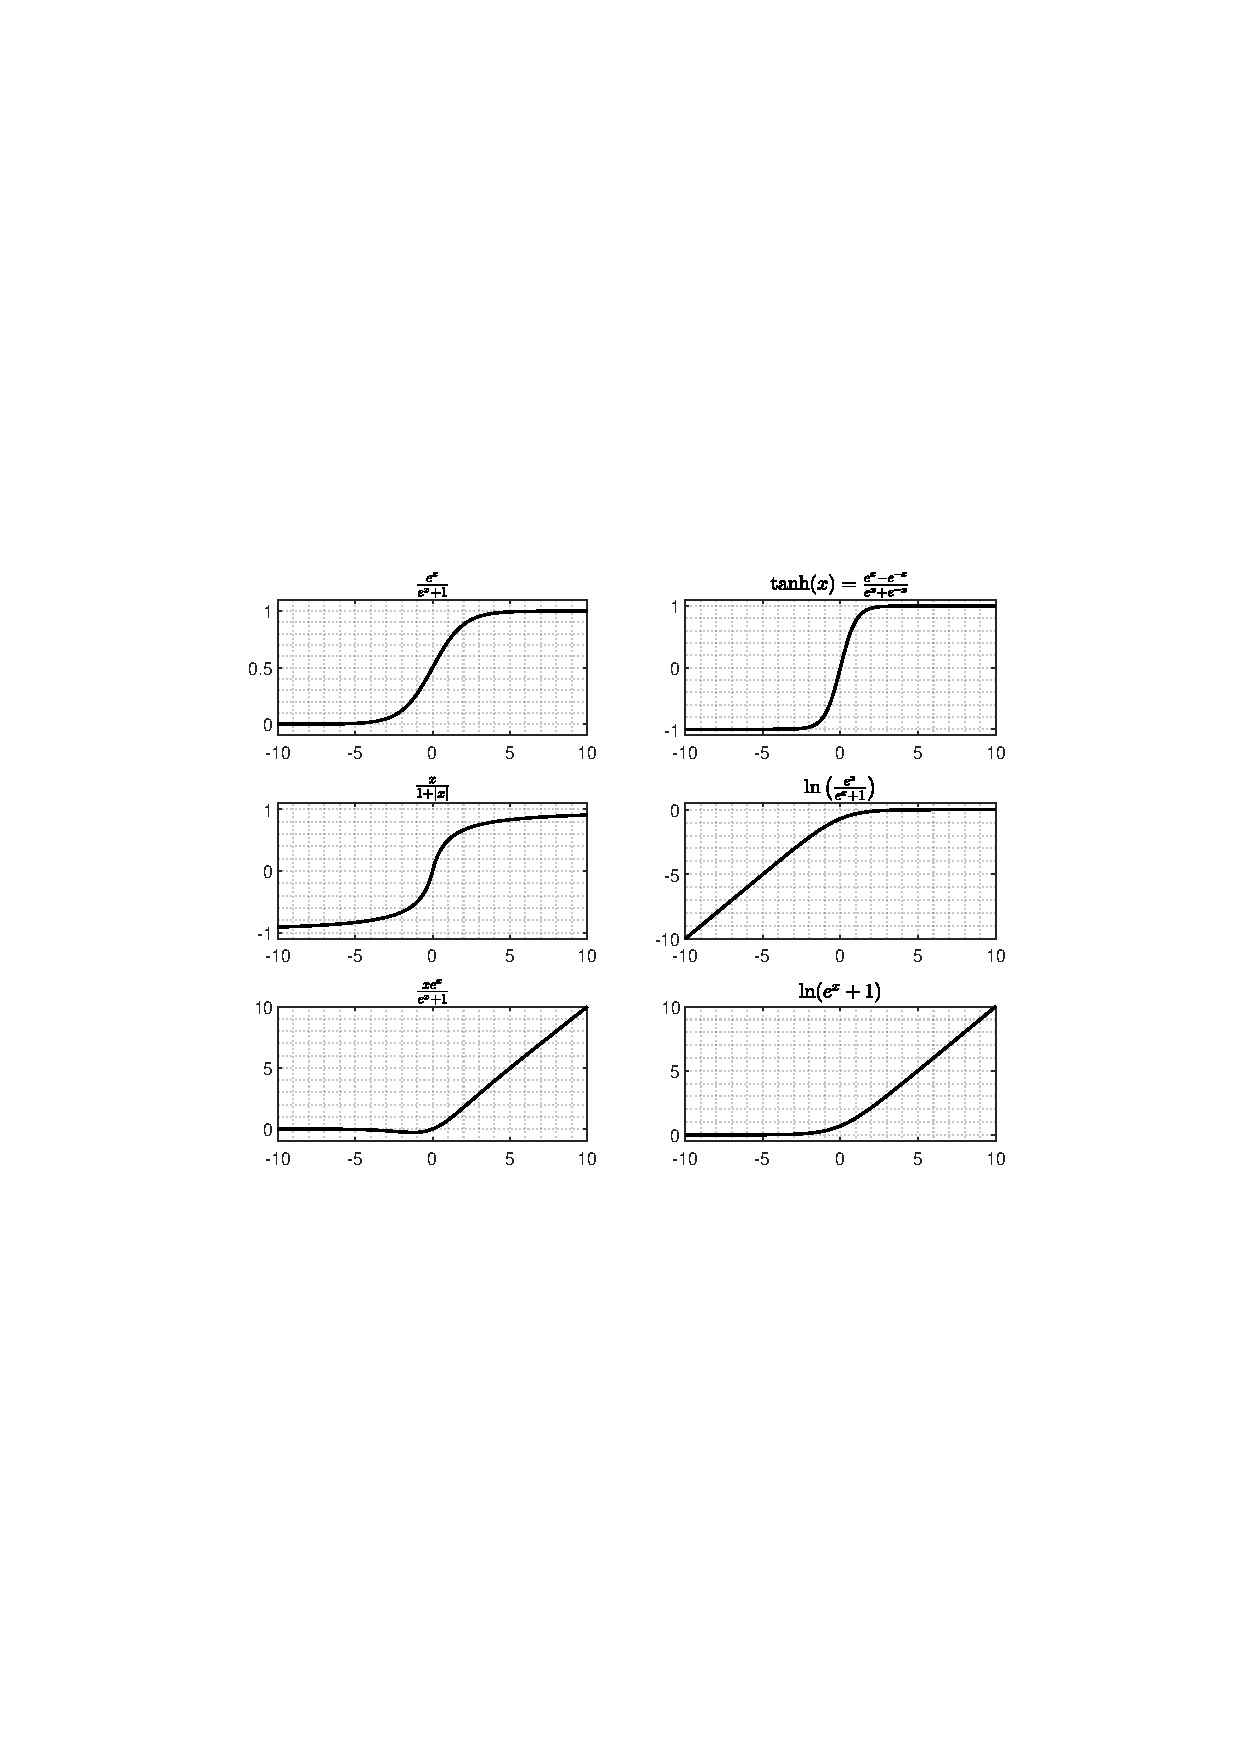
\includegraphics[width=0.95\linewidth]{人工智能函数}
\end{figure} 

\item (2022,新高考II卷)若函数$f(x)$的定义域为
$\mathbf{R}$.且$f(x+y)+f(x-y)=f(x)f(y),\ f(1)=1$,
求$\sum\limits_{k=1}^{22}f(k)$.\\
\textbf{解}\ 令$ x=1,\ y=0 $,有$ f(1)+f(1)=f(1)f(0) $,故$ f(0)=2 $. \\
令$ x=1,\ y=1 $,有$ f(2)+f(0)=f(1)f(1) $,故$ f(2)=-1 $. \\
令$ x=n,\ y=1 $,有$ f(n+1)+f(n-1)=f(n) $,即
\begin{gather}\label{2022II递推数列周期6}
    f(n+1)=f(n)-f(n-1)
\end{gather}
于是,$ f(3)=-2,\ f(4)=-1,\ f(5)=1,\ f(6)=2 $. \\
把(\ref{2022II递推数列周期6})式中的$ n $换成$ n+1 $,有
\begin{gather*}
    f(n+2)=f(n+1)-f(n)=f(n+1)-[f(n+1)+f(n-1)]=-f(n-1)
\end{gather*}
再把$ n $换成$ n+1 $,有$ f(n+3)=-f(n) $,把$ n $换成$ n+3 $,有
\begin{gather*}
    f(n+6)=-f(n+3)=f(n)
\end{gather*}
所以,数列$ f(n) $的周期是6. 又因为$ \sum\limits_{k=1}^{6}f(k)=0 $,
所以
\begin{gather*}
    \sum\limits_{k=1}^{22}f(k)=f(19)+f(20)+f(21)+f(22)=
    f(1)+f(2)+f(3)+f(4)=-3
\end{gather*}
\textbf{注}:递推关系(\ref{2022II递推数列周期6})对应的特征方程为$ x^2=x-1 $,
特征根为$ x_{1,2}=\dfrac{1}{2}\pm \dfrac{\sqrt{3}}{2}\i=
\cos\dfrac{\pi}{3}\pm \i\sin\dfrac{\pi}{3} $,
周期$ T=\dfrac{2\pi}{\frac{\pi}{3}}=6 $. 
设$ f(n)=A\cos\left(\dfrac{n\pi}{3}+\varphi\right) $,
则$ f(0)=A\cos\varphi=2 $,
\begin{gather*}
    f(1)=A\cos\left(\dfrac{\pi}{3}+\varphi\right)=
    \dfrac{1}{2}A\cos\varphi+\dfrac{\sqrt{3}}{2}A\sin\varphi=1
\end{gather*}
所以,$ \sin\varphi=0 $,不妨取$ \varphi=0 $,那么$ A=2 $,
$ f(n) $的通项公式为$ 2\cos\left(\dfrac{n\pi}{3}\right) $. 

此题的背景是:
\begin{gather*}
    \dfrac{1}{\lambda}\cos(x+y)+\dfrac{1}{\lambda}\cos(x-y)=
    \dfrac{2}{\lambda}\cos x\cos y=
    2\lambda\left(\dfrac{1}{\lambda}\cos x\right)
    \left(\dfrac{1}{\lambda}\cos y\right)
\end{gather*}
即$ \dfrac{1}{\lambda}\cos x $满足函数方程$ f(x+y)+f(x-y)=2\lambda f(x)f(y) $. 

\item \label{分式线性变换保交比例题}
给定4个实数$ x_1,x_2,x_3,x_4 $,其中任意两个都不相等,设
$ y_i=\dfrac{ax_i+b}{cx_i+d} $,$ (ad-bc\neq 0,\ i=1,2,3,4) $,求证:
\begin{gather}\label{分式线性变换保交比}
    \dfrac{(y_1-y_3)(y_2-y_4)}{(y_1-y_4)(y_2-y_3)}=
    \dfrac{(x_1-x_3)(x_2-x_4)}{(x_1-x_4)(x_2-x_3)}
\end{gather}
\textbf{证}\ 设$ i\neq j,\ (i,j=1,2,3,4) $,有
\begin{gather*}
    y_i-y_j=\dfrac{ax_i+b}{cx_i+d}-\dfrac{ax_j+b}{cx_j+d}=
    \dfrac{(ad-bc)(x_i-x_j)}{(cx_i+d)(cx_j+d)}
\end{gather*}
\begin{align*}
    \dfrac{(y_1-y_3)(y_2-y_4)}{(y_1-y_4)(y_2-y_3)} &=
    \dfrac{\dfrac{(ad-bc)(x_1-x_3)}{(cx_1+d)(cx_3+d)}\cdot
        \dfrac{(ad-bc)(x_2-x_4)}{(cx_2+d)(cx_4+d)}}{
        \dfrac{(ad-bc)(x_1-x_4)}{(cx_1+d)(cx_4+d)}\cdot
        \dfrac{(ad-bc)(x_2-x_3)}{(cx_2+d)(cx_3+d)} } \\
    &=\dfrac{(x_1-x_3)(x_2-x_4)}{(x_1-x_4)(x_2-x_3)}
\end{align*}

\item 设$ f(x)=\dfrac{ax+b}{cx+d},\ (ad-bc\neq 0) $,若对任意实数
$ x\ (cx+d\neq 0) $,都有$ f(f(x))=x $,求$ a,b,c,d $应满足的条件。\\
\textbf{解}\ 
\begin{gather*}
    f(f(x))=\dfrac{a\cdot\dfrac{ax+b}{cx+d}+b}{c\cdot
        \dfrac{ax+b}{cx+d}+d}=
    \dfrac{(a^2+bc)x+(a+d)b}{(a+d)cx+bc+d^2}=
    \dfrac{x+\dfrac{(a+d)b}{a^2+bc}}{\dfrac{(a+d)c}{a^2+bc}
        \cdot x+ \dfrac{bc+d^2}{a^2+bc}}=x
\end{gather*}
所以,
\begin{align*}
    \left\{
    \begin{aligned}
        (a+d)b=0\q  & \mycircled{1} \\
        (a+d)c=0\q  & \mycircled{2} \\
        \dfrac{bc+d^2}{a^2+bc}=1\q  & \mycircled{3} \\
        ad-bc\neq 0\q  & \mycircled{4}
    \end{aligned}
    \right.
\end{align*}
由\mycircled{3}得:$ a^2=d^2 $. \\
(1) 若$ a=d=0,\ bc\neq 0 $,则$ f(x)=\dfrac{b}{cx} $;\\
(2) 若$ a=d\neq 0 $,由\mycircled{1}、\mycircled{2}可得
$ b=c=0 $,则$ f(x)=x $;\\
(3) 若$ a=-d\neq 0,\ -a^2-bc\neq 0 $,则$ f(x)=\dfrac{ax+b}{cx-a} $.

% QuadraticFractionalLinearTransformation.m
\item 设$a\neq 0$,考虑二次方程$ax^2+bx+c=0$,\\
(1) 令$x=At+B$,其中$A,B$为常数且$A\neq0$,
将原来关于$x$的二次方程转化为关于$t$的二次方程,
求关于$ t $的方程的判别式。\\
(2) 令$x=\dfrac{At+B}{Ct+D}$,其中$A,B,C,D$为常数且$AD-BC\neq0$,
将原来关于$x$的二次方程转化为关于$t$的二次方程,
求关于$ t $的方程的判别式。\\
\textbf{解}\ (1) $aA^2t^2+(2aAB+bA)t+aB^2+bB+c=0$,
$\Delta_1=A^2(b^2-4ac)$. \\
(2) $ (aA^2+bAC+cC^2)t^2+[2aAB+b(AD+BC)+2cCD]t+aB^2+bBD+cD^2=0 $,
\begin{gather}\label{二次方程分式线性变换}
    \Delta_2=(AD-BC)^2(b^2-4ac)
\end{gather} 

\item 求$ f(x)=\dfrac{(x+2)(x+3)}{x+1} $和$ g(x)=\dfrac{x+1}{(x+2)(x+3)} $的值域。\\
\textbf{方法一}\ 换元,令$ t=x+1\neq 0 $,则$ f(x)=f(t-1)=\dfrac{(t+1)(t+2)}{t}=t+
\dfrac{2}{t}+3\in (-\infty,3-2\sqrt{2}]\cup [3+2\sqrt{2},+\infty) $. 
$ g(x)=\dfrac{1}{f(x)}\in (-\infty,3-2\sqrt{2}]\cup [3+2\sqrt{2},+\infty) $. \\
\textbf{方法二}\ 判别式法,两者判别式一样,均为$ \Delta=y^2-6y+1\geq 0,\ y
\in (-\infty,3-2\sqrt{2}]\cup [3+2\sqrt{2},+\infty) $ .

\item 已知$ a $是实数,函数$ f(x)=ax^2+2x-6-4a $,如果$ f(x) $在区间
$ [0,4] $上有零点,求$ a $的取值范围。 \\
\textbf{方法一}\ 
\mycircled{1} 先考虑$ f(x) $在区间$ [0,4] $上有且仅有一个零点,此时$ f(0)\cdot 
f(4)\leq 0 $,(无需区分是一次函数还是二次函数),解得
\begin{gather} \label{根的分布-解集1}
    a\leq -\dfrac{3}{2},\ a\geq -\dfrac{1}{6}
\end{gather}
\mycircled{2} 再考虑$ f(x) $在区间$ [0,4] $上有两个零点,此时必有
$ a\neq 0,\ \Delta=4+4a(6+4a)\geq 0 $,解得
\begin{gather} \label{根的分布-解集2}
    a\leq\dfrac{-3-\sqrt{5}}{4}\approx -1.3090,\ a\geq\dfrac{-3+\sqrt{5}}{4}
    \approx -0.1910,\ a\neq 0
\end{gather}
若$ a>0 $,则$ f(0)=-6-4a<0 $,$ f(x) $在区间$ [0,4] $上不可能有两个零点。\\
若$ a<0 $,则需满足 $ f(0)\leq 0, f(4)\leq 0, 0\leq -\dfrac{2}{2a} \leq 4 $,
解得
\begin{gather} \label{根的分布-解集3}
    -\dfrac{3}{2} \leq a \leq -\dfrac{1}{4}
\end{gather}
(\ref{根的分布-解集2})式和(\ref{根的分布-解集3})式求交集,然后和
(\ref{根的分布-解集1})式求并集,可得$ a $的范围是:
$ \left(-\infty,\dfrac{-3-\sqrt{5}}{4}\right]\cup 
\left[-\dfrac{1}{6},+\infty \right) $. 
\\ 
\textbf{方法二}\ 分离参数,$ a=\dfrac{6-2x}{x^2-4} $,问题转化成求函数
$ y=\dfrac{6-2x}{x^2-4} $在$ [0,4] $上的值域,可以直接求导,也可作代换
$ t=3-x\in[-1,3] $,则$ \dfrac{6-2x}{x^2-4}=\dfrac{2t}{(3-t)^2-4}=
\dfrac{2t}{t^2-6t+5}=\dfrac{2}{t-6+\dfrac{5}{t}} \in 
\left(-\infty,\dfrac{-3-\sqrt{5}}{4}\right]\cup 
\left[-\dfrac{1}{6},+\infty \right) $. \\
\textbf{说明}\ 下面介绍三次曲线$y=f(x)=\dfrac{x+C}{x^2+Ax+B}$的图像该如何手工绘制。\\
(一) 因为$y=f(x)=\dfrac{x+C}{x^2+Ax+B}$的分母是二次,分子是一次,
当$x$充分大时,二次函数的绝对值可以远远大于一次函数的绝对值。所以当$x$趋于
$+\infty$或$-\infty$时,$f(x)$趋于0,即曲线$y=f(x)$必然以$x$轴为渐近线。\\
(二) 曲线$y=f(x)$在$x=-C$处必然会穿越$x$轴。\\
(三) 当$x^2+Ax+B=0$有两个不等实根时,
曲线$y=f(x)$在这两个实根处各有一条垂直渐近线;
当$x^2+Ax+B=0$有两个相等实根时,曲线$y=f(x)$只在实根处有一条垂直渐近线;
当$x^2+Ax+B=0$没有实根时,曲线$y=f(x)$不存在垂直渐近线。\\
(四) $f(x)$的正负号与$g(x)=(x+C)(x^2+Ax+B)$的正负号一致(除了使$x^2+Ax+B=0$的点。)\\
(五) 设$x^2+Ax+B=0$有两个不等实根$x_1,x_2\ (x_1<x_2)$,
如果$-C$位于区间$(x_1,x_2)$外部,则曲线$y=f(x)$在区间$(x_1,x_2)$内有一个极值点,
在$x=-C$所在的分支上有另一个极值点;
如果$-C$位于区间$(x_1,x_2)$内部,则曲线$y=f(x)$没有极值点,在区间
$(-\infty,x_1),(x_1,x_2),(x_2,+\infty)$上都是单调的。\\
\\
对于$ y=\dfrac{6-2x}{x^2-4} $,手工绘图时遵循以下步骤:
先绘制两条垂直渐近线$ x=\pm 2 $,再标记出分子的零点$x=3$,然后根据
三次函数$y=(x+2)(x-2)(3-x) $的正负,确定$ y=\dfrac{2(3-x)}{x^2-4} $在区间
$ (-\infty,-2),(-2,2),(2,3),(3,+\infty) $上的正负,在垂直渐近线的左右两侧,
要让曲线分别向$+\infty$和$-\infty$延伸。当$ |x|\to \pm\infty $时,
要让曲线逐渐靠近$ x $轴。其图像如下:
\begin{figure}[h] % cubicCurve_2x3_x_x2_4.m
    \centering
    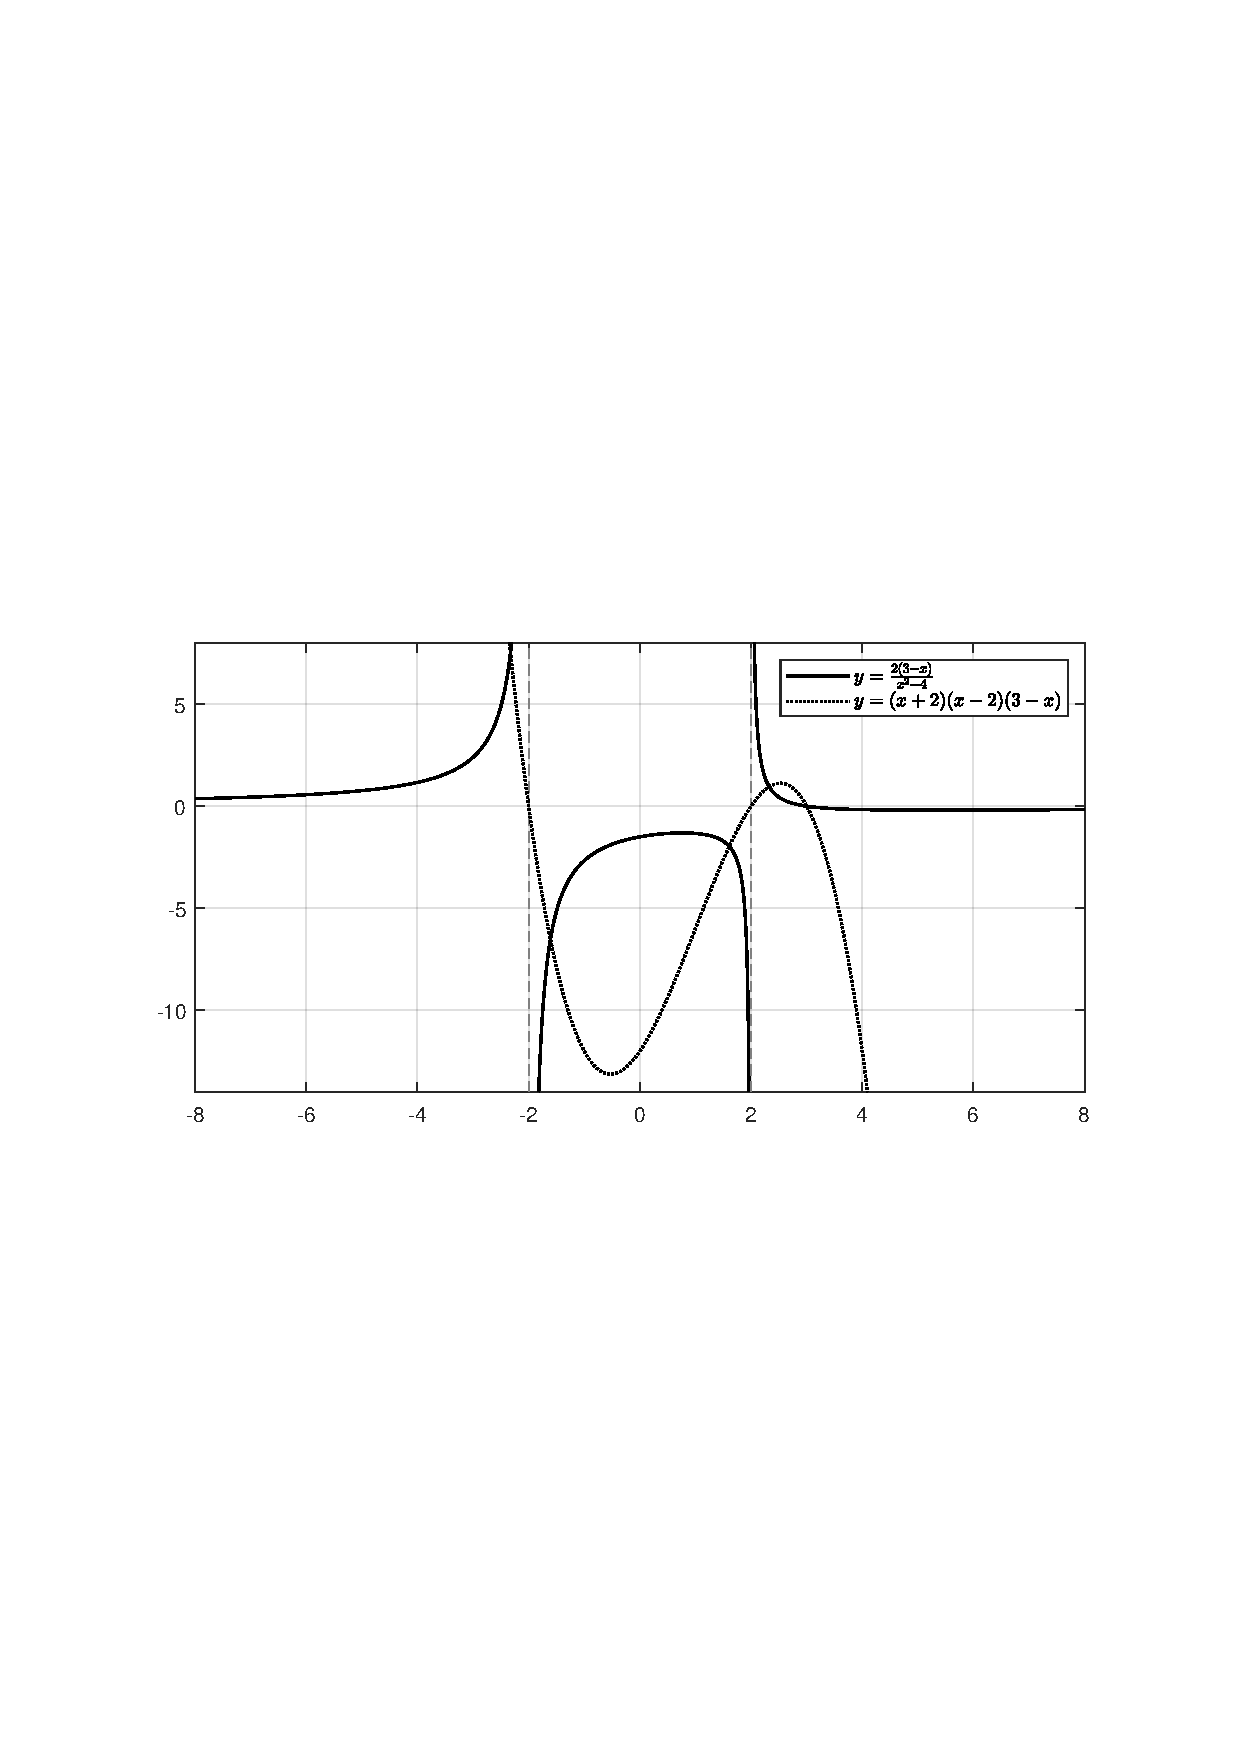
\includegraphics[width=0.7\linewidth]{三次曲线-分子零点在右侧}
\end{figure} \\
$ y=\dfrac{6-2x}{x^2-4} $的分子的零点在分母两个零点所形成的区间的外部,
它在区间$(-2,2)$上有一个极大值点,在区间$(3,+\infty)$上有一个极小值点。\\
而对于$ y=\dfrac{x-1}{x^2-4} $,它的分子的零点在分母两个零点之间,
不存在极值点,在两条垂直渐近线所划分的三个区间中都是单调递减的,其图像如下:
\begin{figure}[h] % cubicCurve_x_1_x2_4.m
    \centering
    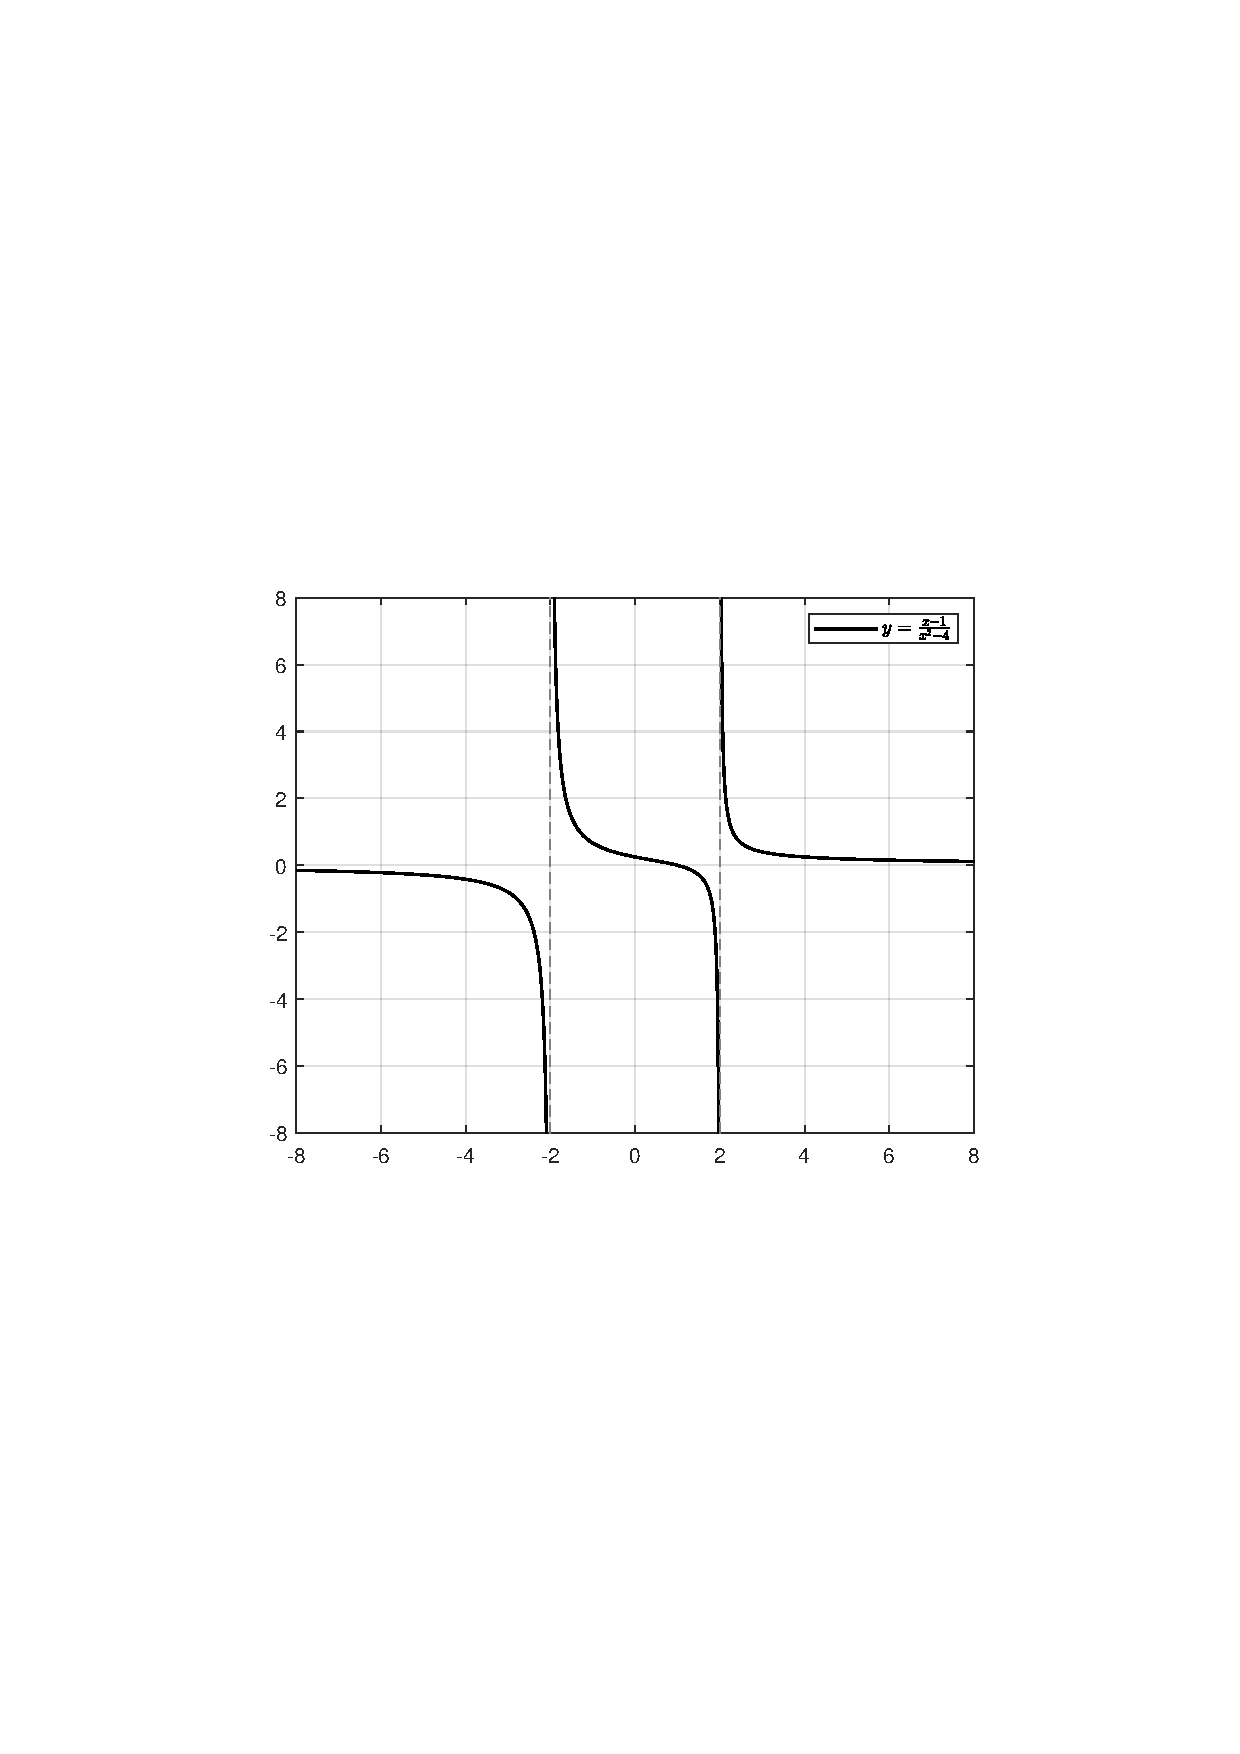
\includegraphics[width=0.45\linewidth]{三次曲线-分子零点在中间}
\end{figure} \\
再展示几种三次曲线的图像如下:
\begin{figure}[h] % CubicCurve3type.m
    \centering
    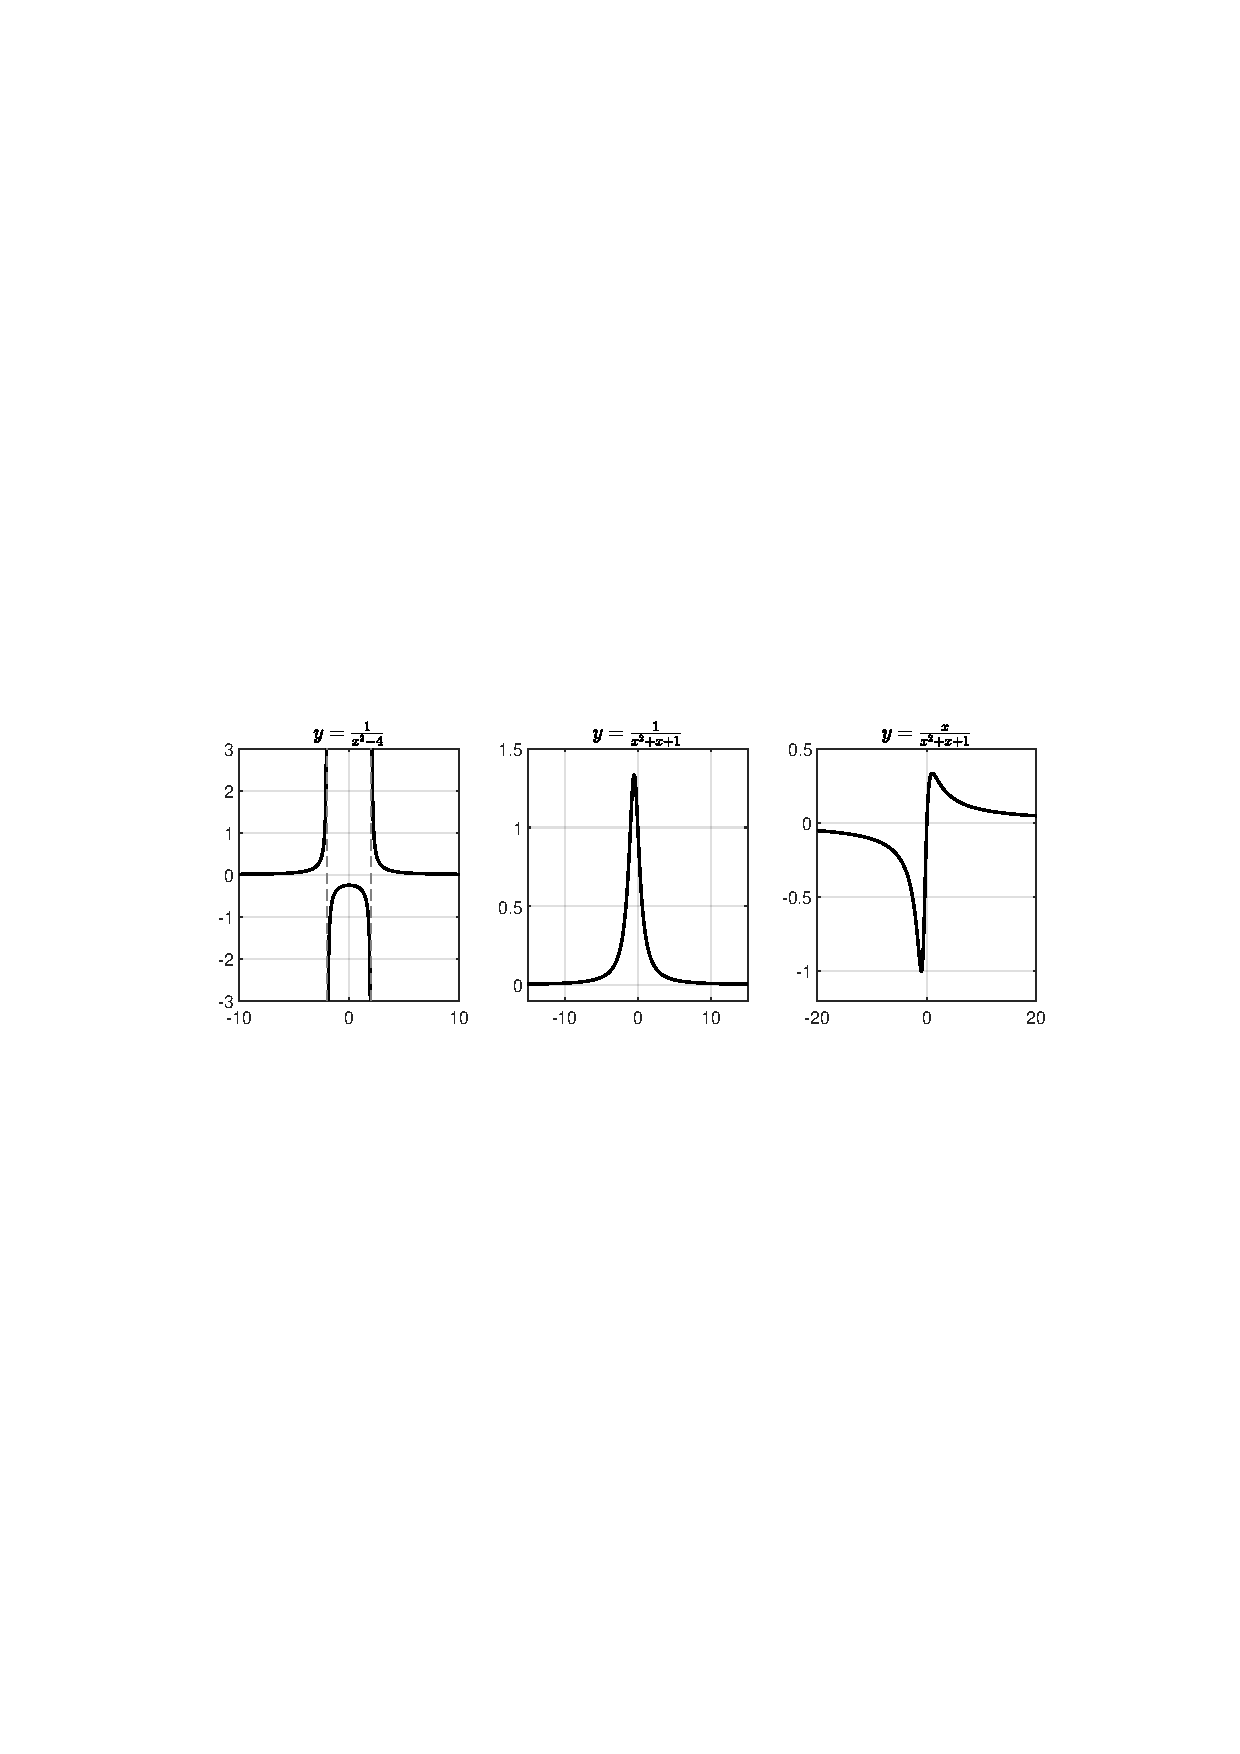
\includegraphics[width=0.84\linewidth]{三次曲线-附加三幅图}
\end{figure} 

\item 已知$ f(x)=x^2+\dfrac{a}{x} $,其中$ a>0 $,若$ f(x) $在
$ [2,+\infty) $上单调递增,求$ a $的取值范围。 \\
\textbf{方法一}\ 任取$ x_1,x_2 $,满足$ 2\leq x_1<x_2 $,那么$ f(x_1)<f(x_2) $,
\begin{align*}
    x_1^2+\dfrac{a}{x_1}-x_2^2-\dfrac{a}{x_2} 
    =(x_1-x_2)\left(x_1+x_2-\dfrac{a}{x_1x_2} \right) <0 
\end{align*} 
所以$ x_1+x_2-\dfrac{a}{x_1x_2}>0,\ a<x_1x_2(x_1+x_2) $. 又因为
$ x_1x_2(x_1+x_2)>2\cdot 2 \cdot(2+2)=16 $,所以$ 0<a\leq 16 $. \\
\textbf{方法二}\ 求导:$ f'(x)=2x-\dfrac{a}{x^2},f'\left(\sqrt[3]{
    \dfrac{a}{2}} \right)=0,\sqrt[3]{\dfrac{a}{2}}\leq 2,a\leq 16 $. \\
\textbf{方法三}\ 用三变量均值不等式:$ f(x)=x^2+\dfrac{a}{2x}+\dfrac{a}{2x} 
\geq 3\sqrt[3]{x^2\cdot\dfrac{a}{2x}\cdot\dfrac{a}{2x}}=
3\sqrt[3]{\dfrac{a^2}{4}} $. 当$ x^2=\dfrac{a}{2x} $时,等号成立,
剩余步骤同方法二。 \\
\textbf{说明}\ $ y=x^2+\dfrac{a}{x}\ (a\neq 0) $可变形为$ x^3-xy+a=0 $,属于三次曲线,
取$ a=4 $,则$ y=x^2+\dfrac{4}{x} $的图像如下:\\
\begin{figure}[h] % cubicCurve_x2T4_x.m
    \centering
    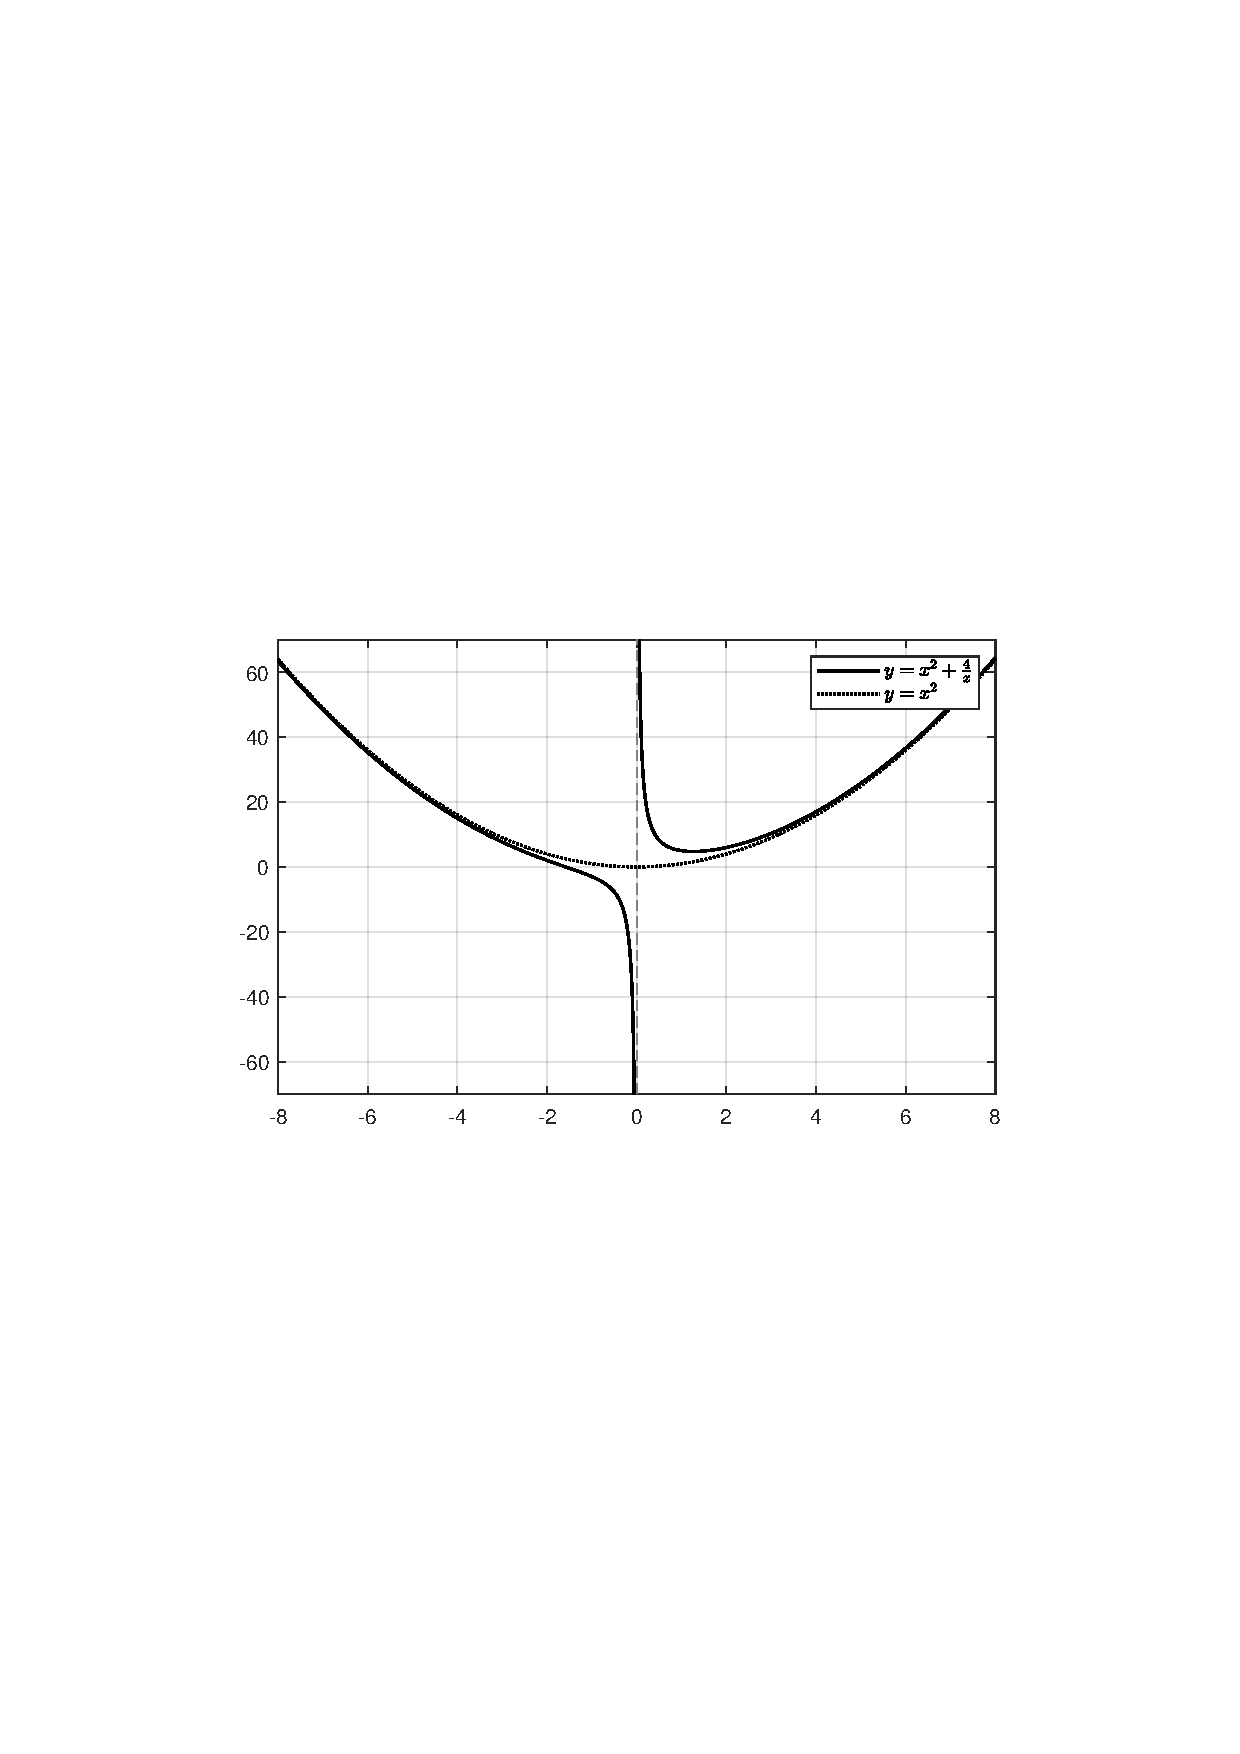
\includegraphics[width=0.5\linewidth]{三次曲线x2y-xy+4}
\end{figure} 

% FenShiHanshu_SanCiQuXian.m
\item 已知$ f(x)=x+\dfrac{a}{x^2} $,其中$ a>0 $,若$ f(x) $在
$ [2,+\infty) $上单调递增,求$ a $的取值范围。 \\
\textbf{方法一}\ 任取$ x_1,x_2 $,满足$ 2\leq x_1<x_2 $,那么$ f(x_1)<f(x_2) $,
\begin{align*}
    x_1+\dfrac{a}{x_1^2}-x_2-\dfrac{a}{x_2^2} 
    =(x_1-x_2)\left[1-\dfrac{a(x_1+x_2)}{x_1^2x_2^2} \right] <0 
\end{align*} 
所以$ 1-\dfrac{a(x_1+x_2)}{x_1^2x_2^2}>0,\ a<\dfrac{x_1^2x_2^2}{x_1+x_2}=
\dfrac{1}{\dfrac{1}{x_1x_2}\left(\dfrac{1}{x_1}+\dfrac{1}{x_2}\right)} $,
又因为$ \dfrac{1}{x_1x_2}\left(\dfrac{1}{x_1}+\dfrac{1}{x_2}\right) $随
$ x_1 $和$ x_2 $都是单调递减的,所以$ \dfrac{x_1^2x_2^2}{x_1+x_2} $随
$ x_1 $和$ x_2 $都是单调递增的,$ \dfrac{x_1^2x_2^2}{x_1+x_2}>
\dfrac{2^2\cdot 2^2}{2+2}=4 $. 于是,$ 0<a\leq 4 $. \\
\textbf{方法二}\ 求导:$ f'(x)=1-\dfrac{2a}{x^3},f'\left(\sqrt[3]{
    2a} \right)=0,\sqrt[3]{2a}\leq 2,\ 0<a\leq 4 $. \smallskip \\
\textbf{方法三}\ 用三变量均值不等式:$ f(x)=\dfrac{x}{2}+\dfrac{x}{2}+\dfrac{a}{x^2}
\geq 3\sqrt[3]{\dfrac{x}{2}\cdot\dfrac{x}{2}\cdot \dfrac{a}{x^2}}=
3\sqrt[3]{\dfrac{a}{4}} $. 当$ \dfrac{x}{2}=\dfrac{a}{x^2} $时,等号成立,
剩余步骤同方法二。 \\
\textbf{说明}\ $ y=x+\dfrac{a}{x^2}\ (a\neq 0) $可变形为$ x^3-x^2y+a=0 $,
属于三次曲线,它有两条渐近线,第一条是$ y=x $,第二条是$ x=0 $. 
取$ a=4 $,则$ y=x+\dfrac{4}{x^2} $的图像如下:
\begin{figure}[h]
    \centering
    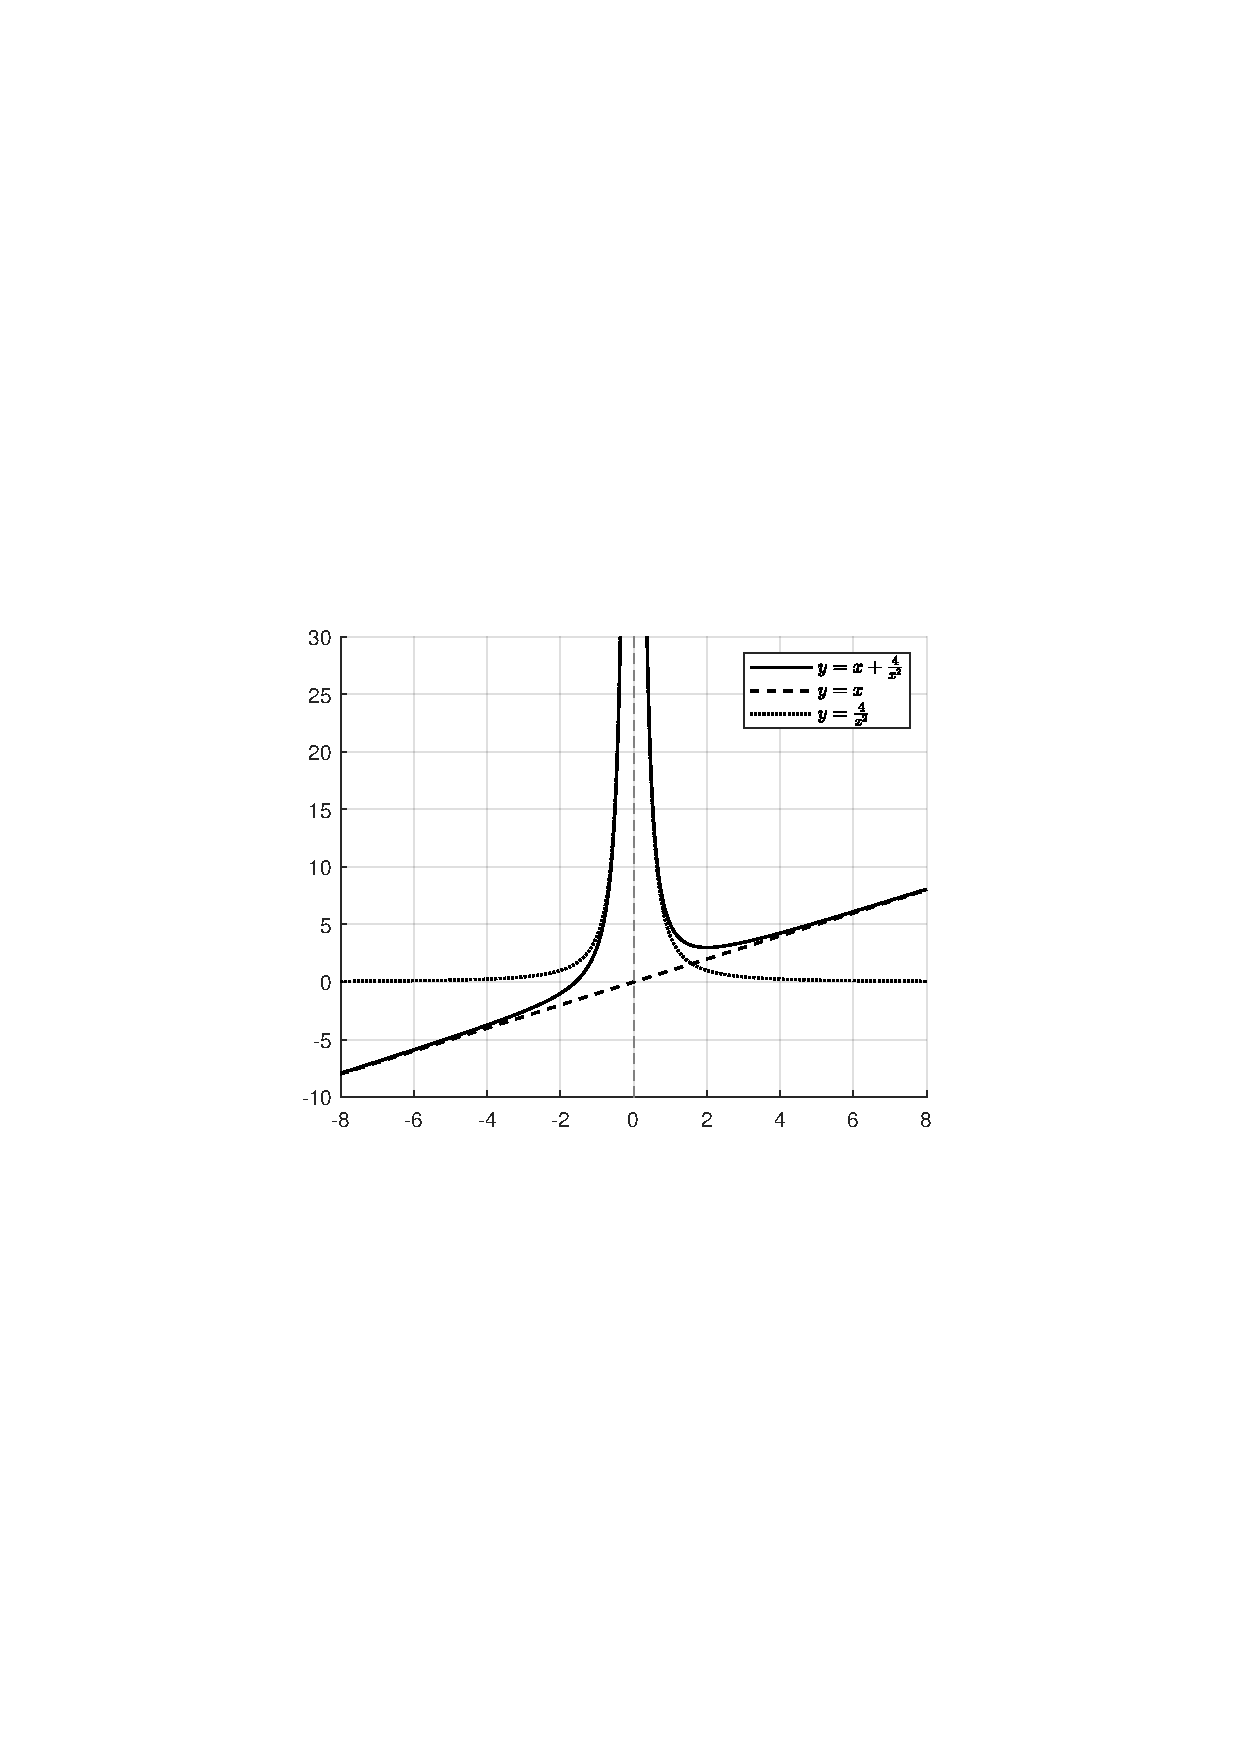
\includegraphics[width=0.5\linewidth]{三次曲线x3-x2y+4}
\end{figure} \\
更一般地,对于$ f(x)=x^m+\dfrac{a}{x^n},\ x>0,\ a>0,\ m,n\in \textbf{N}^+ $,那么
\begin{align*}
    x^m+\dfrac{a}{x^n}=&\ \underbrace{\left(\frac{1}{n}x^m+\frac{1}{n}x^m+\cdots+
        \frac{1}{n}x^m \right)}_{n\text{个}}+
    \underbrace{\left(\frac{1}{m}\frac{a}{x^n}+\frac{1}{m}\frac{a}{x^n}
     +\cdots+ \frac{1}{m}\frac{a}{x^n} \right)}_{m\text{个}}  \\
    \geq &\ (n+m) \left[\left(\frac{1}{n}x^m\right)^n\cdot 
    \left(\frac{1}{m}\dfrac{a}{x^n}\right)^m\right]^{\frac{1}{n+m}} 
    =(n+m) \left(\frac{a^m}{n^nm^m}\right)^{\frac{1}{n+m}}
\end{align*}
当$ \dfrac{1}{n}x^m=\dfrac{1}{m}\dfrac{a}{x^n},\ 
x=\left(\dfrac{na}{m}\right)^{\frac{1}{n+m}} $时,等号成立。\\

\item 已知$ 3f(x)+2f\Big(\dfrac{1}{x}\Big)=x \quad (x\neq 0) $,求$ f(x) $. \\
\textbf{解}\ 
\begin{align*}
    \left\{
    \begin{aligned}
        & 3f(x)+2f\left(\frac{1}{x}\right)=x \\
        & 3f\left(\frac{1}{x}\right)+2f(x)=\frac{1}{x}\quad 
        (\text{把上式的$ x $换成$ \frac{1}{x} $})
    \end{aligned}
    \right.
\end{align*}
解得$ f(x)=\dfrac{3x}{5}-\dfrac{2}{5x} $.  

\item (2008,陕西高考)定义在\textbf{R}上的函数$ f(x) $满足$ f(x_1+x_2)= f(x_1)+f(x_2)+2 x_1x_2 $,
其中$ x_1,x_2\in \textbf{R} $,已知$ f(1)=2 $,求$ f(-3) $. \\
\textbf{方法一}\ 因为满足$ f(x_1+x_2)= f(x_1)+f(x_2)+2\lambda x_1x_2 $的函数是$ f(x)=\lambda x^2+\mu x $,对本题而言就是$ f(x)=x^2+\mu x $,根据$ f(1)=2 $可确定$ \mu=1 $,于是$ f(x)=x^2+x,\ f(-3)=(-3)^2-3=6 $. \\
\textbf{方法二}\ 令$ x_1=x_2=0 $可得$ f(0)=2f(0)+0 $,所以$ f(0)=0 $. 取$ x_1=3,\ x_2=-3 $,于是,
\begin{gather*}
    0=f(3+(-3))=f(3)+f(-3)+2\times 3\times (-3)=f(3)+f(-3)-18 \\
    f(3)=f(1+2)=f(1)+f(2)+4=f(1)+[f(1)+f(1)+2]+4=3f(1)+6=12
\end{gather*}
所以,$ f(-3)=18-f(3)=6 $. 

\item 设$ n $为大于1的正整数,求$ f(x)=\sin^{2n}x+\cos^{2n}x $的值域。\\
\textbf{解}\ 
\begin{align*}
    \sin^{4}x+\cos^{4}x =&\ (\sin^{2}x+\cos^{2}x)^2-2\sin^{2}x\cos^{2}x\\
    =&\ 1-\dfrac{1}{2}\sin^2 2x\in\left[\dfrac{1}{2},1\right] \\
    \sin^{6}x+\cos^{6}x =&\ (\sin^{2}x+\cos^{2}x)^3
    -3\sin^{2}x\cos^{2}x (\sin^{2}x+\cos^{2}x) \\
    =&\ 1-\dfrac{3}{4}\sin^2 2x\in\left[\dfrac{1}{4},1\right] \\
    \sin^{8}x+\cos^{8}x =&\ (\sin^{2}x+\cos^{2}x)^4
    -4\sin^{2}x\cos^{2}x (\sin^{4}x+\cos^{4}x)-6\sin^{4}x\cos^{4}x\\
    =&\ 1-\sin^2 2x\left(1-\dfrac{1}{2}\sin^2 2x\right)
    -\dfrac{3}{8}\sin^4 2x \\
    =&\ \dfrac{1}{8}\sin^4 2x-\sin^2 2x+1 
    \in\left[\dfrac{1}{8},1\right]
\end{align*}
可以猜想:$ f(x)=\sin^{2n}x+\cos^{2n}x $的值域是
$ \left[\dfrac{1}{2^{n-1}},1\right] $. \\
因为$ \sin^2 x,\cos^2 x\in[0,1] $,所以
\begin{gather*}
    \sin^{2n}x\leq \sin^2 x ,\q \cos^{2n}x\leq \cos^2 x  \\ \sin^{2n}x+\cos^{2n}x\leq \sin^{2}x+\cos^{2}x=1
\end{gather*}
当$ \sin^2 x=0 $或1时,以上等号成立。\\
再利用幂函数$ g(x)=x^n $的凹凸性,那么
\begin{gather*}
    \dfrac{g(\sin^2 x)+g(\cos^2 x)}{2}\geq g\left(
    \dfrac{\sin^2 x+\cos^2 x}{2}\right)=\dfrac{1}{2^n} \\
    f(x)=g(\sin^2 x)+g(\cos^2 x)\geq \dfrac{1}{2^{n-1}}
\end{gather*}
当$ |\sin x|=|\cos x|=\dfrac{\sqrt{2}}{2} $时,以上等号成立。

\item $ ^* $ $ x_1+x_2+x_3=1,\ x_1^2+x_2^2+x_3^2=2,\ 
x_1^3+x_2^3+x_3^3=3 $,求$ x_1x_2x_3 $. \\
\textbf{解}\ 
\begin{align*}
    (x_1+x_2+x_3)^2-(x_1^2+x_2^2+x_3^2)=&\ 2(x_1x_2+x_2x_3+x_1x_3)=1-2=-1\\
    x_1x_2+x_2x_3+x_1x_3=&\ -\frac{1}{2} 
\end{align*}
\begin{align*}
     &\ (x_1+x_2+x_3)^3-(x_1^3+x_2^3+x_3^3)=1-3=-2 \\
    =&\ 3(x_1^2x_2+x_1x_2^2+x_1^2x_3+x_1x_3^2+x_2^2x_3+x_2x_3^2)+6x_1x_2x_3\\
    =&\ 3(x_1x_2+x_1x_3+x_2x_3)(x_1+x_2+x_3)-3x_1x_2x_3
    =-\frac{3}{2}-3x_1x_2x_3
\end{align*}
或者
\begin{align*}
    & x_1^3+x_2^3+x_3^3-3x_1x_2x_3=3-3x_1x_2x_3  \\
    =&\  (x_1+x_2+x_3)(x_1^2+x_2^2+x_3^2-x_1x_2-x_2x_3-x_3x_1)\\
    =&\  1\cdot\left(2+\dfrac{1}{2}\right)=\frac{5}{2}
\end{align*}
于是$ x_1x_2x_3=\dfrac{1}{6} $. 

根据韦达定理,$ x_1,x_2,x_3 $实际上是三次方程$ x^3-x^2-\dfrac{1}{2}x-
\dfrac{1}{6}=0 $的三个根,
借助求根公式可算出:$ x_1 \approx 1.430849566,x_{2,3}\approx -0.215424783 
\pm 0.2647131993 i $. 

\end{enumerate}

\section{习题} 
\begin{enumerate}[label={\textbf{\arabic*.}},leftmargin=
    \inteval{\myenumleftmargin}pt]
%\item $ y=\cos(2x^2+3x) $\underline{\hspace{1cm}}(填“是”或“不是”)周期函数。
%$ y=x\cos(\dfrac{1}{x}+1) $\underline{\hspace{1cm}}(填“是”或“不是”)周期函数。
%\ifteach \\
%\textbf{解}\ 不是,不是
%\fi
\item  已知$ x\in \textbf{R} $,求下列函数的最小值。\\
(1)$ |x+1|+|x-3|+|x-5| $;\quad (2) $ |x-1|+|2x-4|+|4x-16| $ .

\item 设$ ac\neq 0 $,尝试绘制$ |ax-b|+|cy-d|=1 $的图像。

\item 比较$ 2^3 $与$ 3^2 $、$ 3^4 $与$ 4^3 $、$ 4^5 $
与$ 5^4 $、$ 5^6 $与$ 6^5 $的大小,猜测一般性规律。

\item 比较$ \log_2 3 $与$ \log_3 4 $的大小,当$ n\geq 2 $时,
猜测$ \log_n (n+1) $与$ \log_{n+1} (n+2) $的大小的一般规律。

\item 证明表\ref{函数迭代列表}中的全部结果。

\item 定义$\ f_1(x)=f(x)=\dfrac{1+x}{1-x},\ f_{n+1}(x)=f(f_n(x)) $,
其中$ n \in \textbf{N}^+ $,求$ f_{2021}(x) $. 

\item 定义数列$ \{a_n\}:\ a_1=2,a_{n+1}=\dfrac{1+a_n}{1-a_n} $,
求$ a_{2022} $. 

\item 已知$ x\geq 0 $,定义$\ f_1(x)=f(x)=x+2\sqrt{x}+1,\ f_{n+1}(x)=
f(f_n(x)) $,求$ f_{50}(49) $. 

\item 定义在$ \textbf{R} $上的偶函数$ f(x) $满足$ f(x)=f(6-x) $,当$ x\in [0,3] $时,
$ f(x)=x^3-8 $,求$ f(1)+f(2)+\cdots +f(2022) $的值。

\item 定义$ f(x)=\dfrac{a^x}{a^x+\sqrt{a}} \ (a>0,a\neq 1)$. \\
(1)求$ f(x)+f(1-x) $;\\
(2)求$ f\left(\dfrac{1}{101}\right)+f\left(\dfrac{2}{101}\right)+
\cdots +f\left(\dfrac{100}{101}\right) $. 

\item 定义在$ \textbf{R} $上的函数$ f(x) $满足
$ f(x+2)=\sqrt{2}f(x+1)-f(x) $,求$ f(x) $的周期。

\item 用尽可能多的方法求以下函数的值域,并手工绘制函数图像,然后用GeoGebra验证
值域和图像。\\
(1)$ y=\dfrac{2x+4}{x^2+x+3},\ x\in \textbf{R} $. \\
(2)$ y=\dfrac{x-1}{x^2-x-2},\ x\in\left[-\dfrac{1}{2},
                            \dfrac{3}{2}\right] $. \\
(3)$ y=\dfrac{x+1}{x^2-3x+2},\ x\neq 1,2 $. \\
(4)$ y=\dfrac{2x-\sqrt{x^2+1}}{2x+\sqrt{x^2+1}},\ x\in (-\infty,0) $. \\
(5)$ y=\dfrac{x}{(x-1)^2},\ x\neq 1 $.

\item 请写出满足以下函数方程并经过给定点的基本初等函数的解析式。\\
(1) $ f\left(\dfrac{1}{4}x_1+\dfrac{3}{4}x_2\right)=\dfrac{1}{4}f(x_1)+
\dfrac{3}{4}f(x_2),\ f(1)=2,\ f(3)=8 $,
则$ f(x)=\underline{\hspace{2cm}} $. \\
(2) $ f(x_1+x_2)=f(x_1)f(x_2),\ f(2)=9 $,
则$ f(x)=\underline{\hspace{2cm}} $. \\
(3) $ f(x_1x_2)=f(x_1)+f(x_2),\ f(5)=1 $,
则$ f(x)=\underline{\hspace{2cm}} $. \\
(4) $ f(x_1x_2)=f(x_1)f(x_2),\ f(3)=27 $,
则$ f(x)=\underline{\hspace{2cm}} $. \\
(5) $ f(x_1+x_2)=f(x_1)+f(x_2)+4x_1x_2,\ f(1)=4 $,
则$ f(x)=\underline{\hspace{2cm}} $.

\item 求解以下函数方程:\\
(1) $ 4f(x)-2f(\dfrac{1}{x})=3x^2 \quad (x\neq 0) $. \\
(2) $ 2f(x)+f(2-x)=x $.  \\
(3) $ 3f(x^3)+2f(-x^3)=4x $. 

\item 因式分解:\\ (1)$ x^3-3x+2 $;\quad (2)$ x^3 + 2x^2 - x - 2 $;  \\
(3)$ x^3 + 3x^2 + 4x + 4 $;\quad (4)$ 2x^3 + 9x^2 + 7x - 6 $ ;\\
再对(4)式写出韦达定理的三个式子。

\item 已知$ a $是实数,函数$ f(x)=ax^2+5x−20-5a $,如果$ f(x) $在区间
$ [0,5] $上有零点,求$ a $的取值范围。

\item (2022,上海春季高考)已知定义在\textbf{R}上的函数$ f(x) $,它在
$ (-\infty,0) $上单调递增,且对任意$ t>0 $,满足$ |f(x+t)-2f(x)+f(x-t)|
=|f(x+t)-f(x)|-|f(x)-f(x-t)| $,求证:$ f(x) $在\textbf{R}上单调递增。 

\item 设$ f(x)\geq 0 $,对任意$ x_1x_2\geq 0 $,都有
$ f(x_1+x_2)=f(x_1)+f(x_2)+2\sqrt{f(x_1)f(x_2)} $,
用数学归纳法证明:对任意非负整数$ n $,都有$ f(nx)=n^2f(x) $.

\item $ ^* $定义在\textbf{R}上的函数$ f(x) $满足$ f(\sqrt{x_1^2+x_2^2})= 
f(x_1)f(x_2) $,其中$ x_1,x_2\in \textbf{R} $,已知$ f(1)=2 $,
求证:$ f(x)=2^{x^2} $.

\end{enumerate}

\section{习题答案}
\begin{enumerate}[label={\textbf{\arabic*.}},leftmargin=
    \inteval{\myenumleftmargin}pt]
\item 三个绝对值里面有三个不同的零点,三个零点把数轴分成4段,每一段上都是单调的
(都是直线),所以最小值只可能在三个零点中的某一零点处取得,
第(1)题当然是在中间零点处达到。
第(2)题只需把$ x=1,2,4 $分别代入计算,即可找出最小值。\\
(1)$ x=3 $时取得最小值6. \quad (2) $ x=4 $时取得最小值7. 


\item 图像是一个以$ \left(\dfrac{b}{a},\dfrac{d}{c}\right) $
为中心的的菱形,菱形的两条对角线分别平行于$ x $轴和$ y $轴。

\item 规律:当$ n\geq 3 $时,$ n^{n+1}>(n+1)^n $. 

\item $ \log_n (n+1) > \log_{n+1} (n+2) $. \\ 因为$ \log_n (n+1)=
\dfrac{\ln (n+1)}{\ln n}=\dfrac{\ln n+\ln\left(1+\frac{1}{n}
    \right)}{\ln n}=1+\dfrac{\ln\left(1+\frac{1}{n}
    \right)}{\ln n} $随$ n $递减。

\item 略

\item 
$ k\in \textbf{N} $, $ f_{4k+1}(x)=\dfrac{1+x}{1-x} $,
$ f_{4k+2}(x)=-\dfrac{1}{x} $, $ f_{4k+3}(x)=\dfrac{x-1}{x+1} $,
$ f_{4k+4}(x)=x $,$ f_{2021}(x)=f_1(x)=\dfrac{1+x}{1-x} $. 

\item 数列的周期为4,$ a_{4k+1}=2,a_{4k+2}=-3,a_{4k+3}
=-\dfrac{1}{2},a_{4k+4}=\dfrac{1}{3},\ a_{2022}=a_2=-3 $. 

\item 3249

\item 
$ f(1)+f(2)+f(3)+f(4)+f(5)+f(6)=f(1)+f(2)+f(3)+f(2)+f(1)+f(0)=-3,\ 
f(1)+f(2)+\cdots +f(2022)=\dfrac{2022}{6}[f(1)+f(2)+\cdots+f(6)]=-1011 $. 

\item 
(1) $ f(x)+f(1-x)=1 $;\quad (2) 50.

\item 
\begin{align*}
    f(x+3) =&\ \sqrt{2}f(x+2)-f(x+1) \\
    =&\  \sqrt{2}[\sqrt{2}f(x+1)-f(x)]-f(x+1) \\
    =&\ f(x+1)-\sqrt{2}f(x) \\
    f(x+4) =&\ \sqrt{2}f(x+3)-f(x+2) \\
    =&\  \sqrt{2}[f(x+1)-\sqrt{2}f(x)]-[\sqrt{2}f(x+1)-f(x)] \\
    =&\ -f(x) \\
    f(x+8)=&\ -f(x+4)=f(x)
\end{align*} 
周期是8.

\item  %ExciseAnswerFunctionFigure.m
\begin{figure}[h]
    \centering
    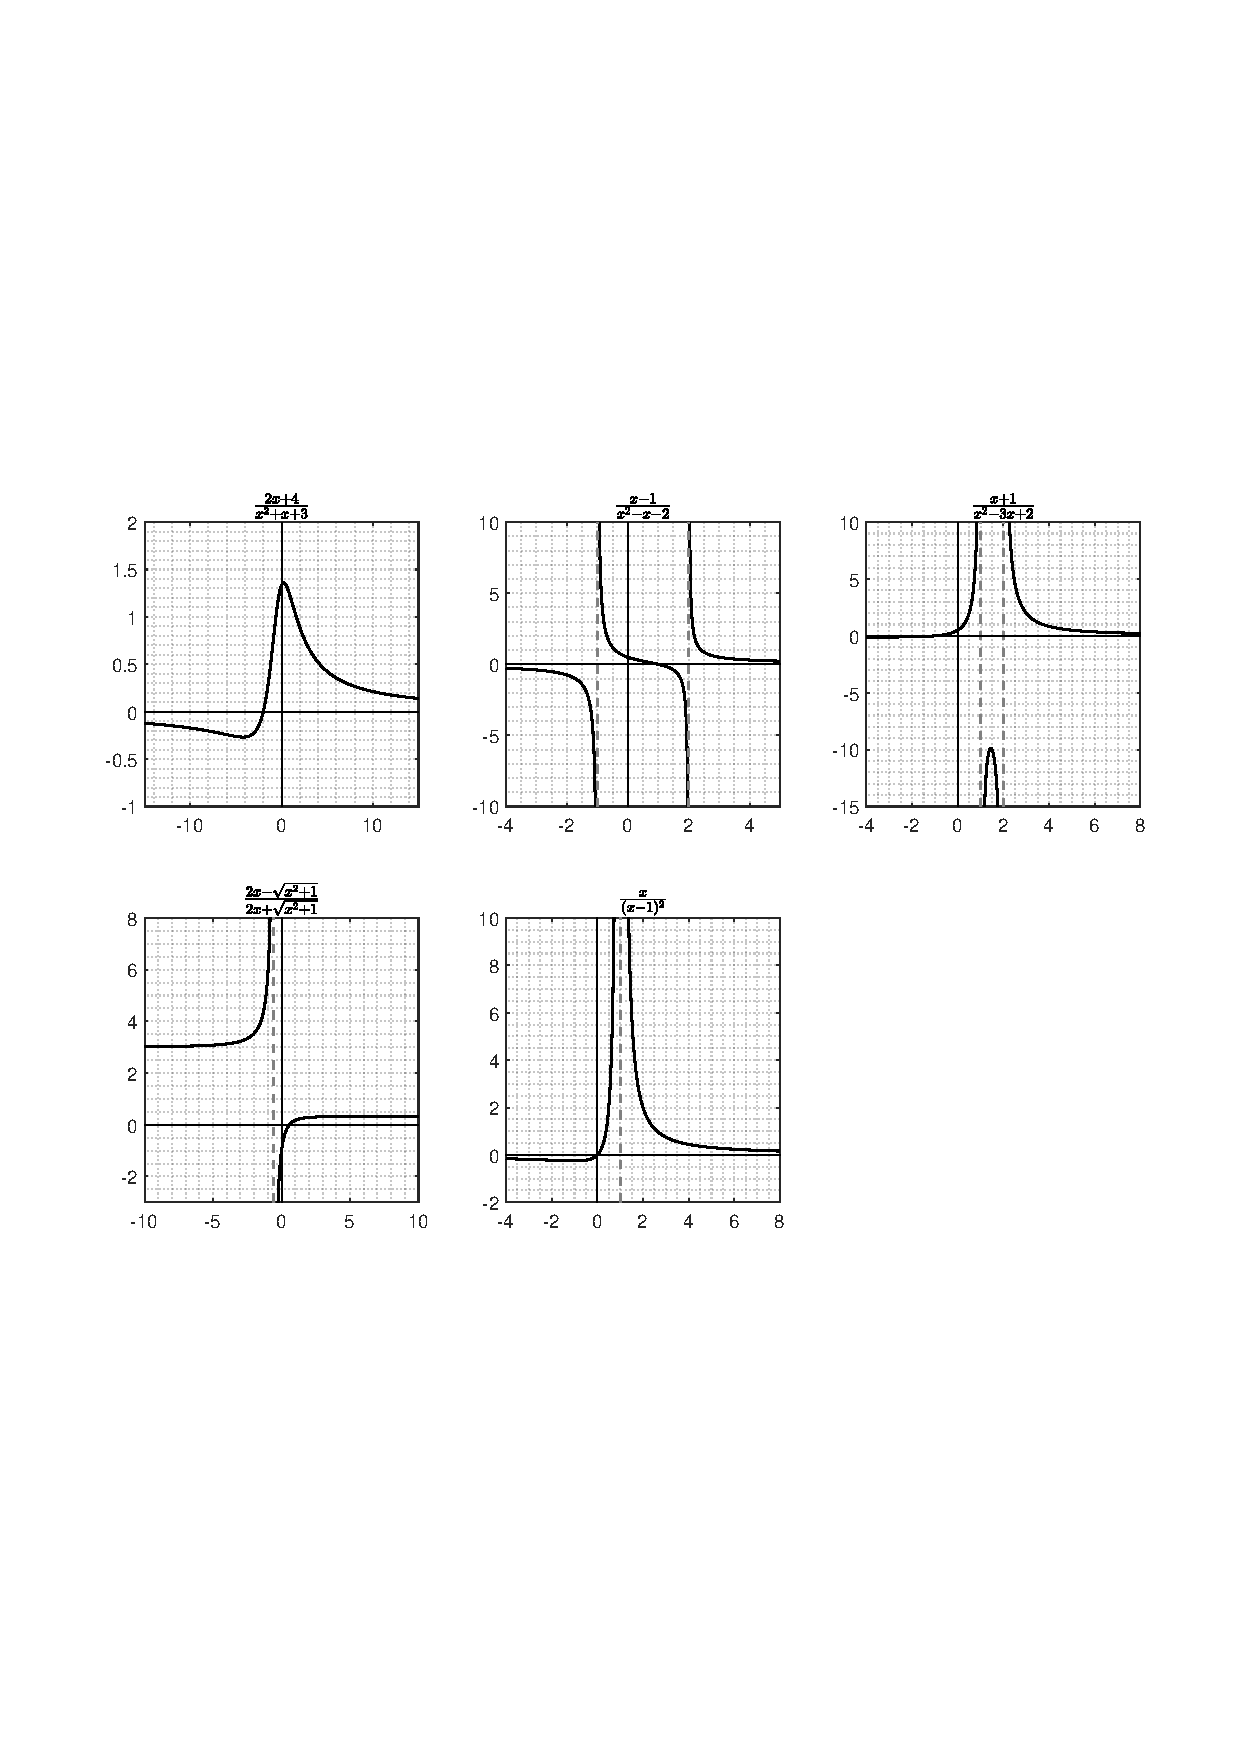
\includegraphics[width=0.95\linewidth]{PDF_Picture/第一章练习题中5个函数图像}
\end{figure}
(1)$ \left[-\dfrac{2}{2\sqrt{5}+3},\dfrac{2}{2\sqrt{5}-3}\right] $. \\
(2)$ \left[-\dfrac{2}{5},\dfrac{6}{5}\right] $. \\
(3)$ \left(-\infty,\dfrac{1}{2\sqrt{6}-5}\right] \cup 
\left[-\dfrac{1}{2\sqrt{6}+5},+\infty\right) $. \\
(4) $ \left(-\infty,-1\right) \cup \left(3,+\infty\right) $. \\
(5) $ \left[-\dfrac{1}{4},+\infty\right) $.

\item (1) $ 3x-1 $;\quad (2) $ 3^x $;\quad 
(3) $ \log_5x $;\quad (4) $ x^3 $ ;\quad (5) $ 2x^2+2x $.

\item 
(1) $ f(x)=x^2+\dfrac{1}{2x^2} $. \\
(2) $ f(x)=x-\dfrac{2}{3} $. \\
(3) $ f(x)=4\sqrt[3]{x} $. 

\item 
(1)$ (x-1)^2(x+2) $  \\
(2)$ (x - 1)(x + 1)(x + 2) $ \\
(3)$ (x^2+x+2)(x+2) $ \\
(4)$ (2x-1)(x+2)(x+3) $ 

\item 
$ \left(-\infty,\dfrac{-4-\sqrt{11}}{2}\right] \cup 
\left[-\dfrac{1}{4},+\infty\right) $. 

\item 取$ a=f(x+t)-f(x),\ b=f(x)-f(x-t) $,依题意,
$ |a-b|=|a|-|b|\geq 0 $,再根据$ |a-b|\geq |a|-|b| $,所以必有 
$ a\geq b \geq 0\ \ \mycircled{1} $或者
$ a\leq b\leq 0\ \ \mycircled{2} $. 下面来说明\mycircled{2}不可能成立。
因为$ f(x+t)-f(x) $始终与$ f(x)-f(x-t) $同号,那么$ f(x+t)-f(x) $
与$ f(x-kt)-f(x-(k+1)t) $同号($ k\in \textbf{N}^+ $).如果存在
$ 0\leq x_1<x_2 $使得$ f(x_1)\geq f(x_2) $,令$ t=x_2-x_1>0 $,
再取充分大的$ k $,使得$ x_1-kt<0 $,那么
\begin{align*}
    & f(x_2)-f(x_1)=f(x_1+t)-f(x_1) \leq 0 \\
    & f(x_1-kt)-f(x_1-(k+1)t)\geq 0\q 
    (\because f(x)\text{在}\ (-\infty,0)\ \text{上单调递增})
\end{align*}
这两个式子符号不一样,产生了矛盾。所以只有\mycircled{1}成立。证毕。

\item 
\begin{align*}
    f((n+1)x)=&\ f(nx+x) \\
    =&\ f(nx)+f(x)+2\sqrt{f(nx)f(x)} \\
    =&\ n^2f(x)+f(x)+2\sqrt{n^2f(x)f(x)} \\
    =&\ (n^2+1+2n)f(x) \\
    =&\ (n+1)^2f(x)
\end{align*}

\item 
显然有$ f(x)=f(-x)=f(|x|) $,用数学归纳法可以证明:$ f(\sqrt{n}x)=[f(x)]^n $,
设$ m,n \in \textbf{N}^+ $,
\begin{gather*}
    f(m)=f(|m|)=f(\sqrt{m^2}\cdot 1)=[f(1)]^{m^2}=2^{m^2} \\
    f(|m|)=f\left(\sqrt{n^2}\left|\dfrac{m}{n}\right|\right)
    =\left[f\left(\left|\dfrac{m}{n}\right|\right)\right]^{n^2}=2^{m^2} \\
    f\left(\dfrac{m}{n}\right)=f\left(\left|\dfrac{m}{n}\right|\right)
    =2^{(\frac{m}{n})^2} \quad (\text{上式两边开} n^2\ \text{次方} )
\end{gather*}
所以题目结论对任意有理数成立,对任意的无理数,可以由函数的连续性推出同样成立。


\end{enumerate}
\myfootnote{\CopyrightStatementChap}

% {\footnotesize (可在以下空白区域自行增补知识点。)}  
\cleardoublepage

%------------------------------------------
